%\documentclass[12pt]{scrreprt}
\documentclass[12pt]{report}

% language may be romanian or english (default is english)
% type may be bachelor or master (default is bachelor)
\usepackage[language=english, type=master]{style}

%\geometry{a4paper,top=2.5cm,left=3cm,right=2.5cm,bottom=2.5cm}
%in style
%controlling the appearance of your headers and footers
\usepackage{fancyhdr}
\pagestyle{fancy}
\lhead{}
\chead{}
\renewcommand{\headrulewidth}{0.2pt}
\renewcommand{\footrulewidth}{0.2pt}

\begin{document}

\specialization{Sisteme informatice avansate}
\title{A Cloud-Based Closed-Loop Payment System with Hybrid On-Chip Reconciliation for Festival Environments}
\author{Tudor Esan}
\supervisor{Assoc. Prof. Christian Sacarea, PhD}

\maketitle


\newpage
\thispagestyle{empty}
\mbox{}
\newpage
\pagenumbering{roman}

\cleardoublepage
ABSTRACT
\vspace{0.5cm}
\hrule
\vspace{0.5cm}
%\cleardoublepage

This thesis describes a cloud-based closed-loop payment system for music festivals and large outdoor events. The system is online by default and uses the bracelet balance as a fallback when the network goes down. Festivals are known for bad connectivity when a lot of people gather in the same place, but in our view, building the whole system around the assumption that the network will fail brings more complexity than it is worth. We keep things online most of the time using a Starlink uplink and a redundant network topology, and we let the NFC wristband hold the balance as a cache for the rest. When the network is up, transactions go through the server in real time. When it is not, the chip itself stores the balance and a monotonic debit counter, so vendor terminals can approve a payment locally and not let anyone spend money twice. As soon as connectivity comes back, the terminals push their queued transactions to the server in batches, and the server applies them against its own credit counter. Credits are written only by the server and debits are written only by the chip, so the two flows meet again on their own when the network is back. We assess the architecture against what a real festival actually needs and we argue that treating offline as a bounded fallback, and not as the foundation of the system, gives a simpler and more maintainable result.

\tableofcontents


\newpage
\pagenumbering{arabic}

\chapter{Introduction}
\label{chap:introduction}

Music festivals and large outdoor events have become a massive part of modern culture. Every summer, millions of people gather in open fields, parks, and temporary venues to enjoy live performances and food. From Untold in Romania to Tomorrowland in Belgium, these events keep growing in size and complexity. But behind all the excitement, there is a very practical problem that organizers have to deal with: how do you let tens of thousands of people buy food, drinks, and merchandise in a place where the internet barely works?

The traditional approach was straightforward: people brought cash, stood in line, and paid at the counter. It was slow, it was messy with always having change and there was always the risk of theft or losing your wallet in the crowd. Over the past decade, many festivals have moved towards cashless payment systems, typically based on RFID wristbands or prepaid cards. The idea is simple: you load money onto your wristband before or during the event, and then you just tap it at a vendor terminal to pay. Industry data from cashless technology providers suggests that RFID systems reduce transaction times by up to 80 percent compared to cash and that festival organizers see average revenue increases of around 22 percent after going cashless \cite{Tappit2024}. These figures are consistent with the academic evidence: a recent meta-analysis across 71 studies found a statistically significant, small positive effect of cashless payments on consumer spending ($g = 0.135$, 95\% CI [0.068; 0.203]), driven primarily by the reduced psychological friction of not physically handing over money \cite{Schomburgk2024}.

However, these systems come with a critical weakness: most of them depend on a reliable internet connection. And if there is one thing that festivals are known for, it is terrible connectivity. When tens of thousands of people gather in the same area, all using their phones simultaneously, the cellular network simply cannot handle the load. Shafiq et al.~\cite{Shafiq2013} conducted the first large-scale characterization of cellular network performance during crowded events using real-world traces from a tier-1 US network. Their findings are impressive: pre-connection failures increased by 100 to 5,000 times compared to routine days, driven by users exhausting the limited bandwidth of the signaling channel when too many devices attempt to acquire radio resources simultaneously. This degradation extended as far as 10 miles around the event venue as attendees arrived and departed. Even for users who managed to connect, voice call failures increased by 7 to 30 times, packet, and round-trip times increased by up to 7 times. The performance spikes were particularly severe during intermissions, when large numbers of attendees simultaneously attempted to use their devices. Notably, the study found that even with portable base stations and free Wi-Fi offloading already deployed, these degradation levels persisted, highlighting a fundamental capacity limitation rather than a simple configuration problem.


This is where things get problematic for payment systems. If the payment terminal at a food stall needs to contact a remote server to authorize a transaction, and the network is down or painfully slow, the transaction fails. The attendee cannot buy food. The vendor loses a sale. Multiply this by tens of thousands of transactions per day, and you can see why this is a serious issue. The most famous example of this going wrong happened at the Download Festival in the UK in 2015, the first major UK festival to go completely cashless. The RFID system experienced technical failures that left attendees unable to purchase food or drinks, with many taking to social media to describe the system as useless. Although organizers claimed only around one percent of attendees were affected, the backlash was severe enough that the festival abandoned the cashless-only approach the following year \cite{eFestivals2016}.

The core question this thesis tries to answer is: can we build a payment system that works reliably at festivals and that does not fall apart when the network has a bad moment? Our approach is to design a system that operates online by default, with connectivity coming from a Starlink uplink and a redundant network topology, so that vendor terminals can talk to the cloud backend in real time most of the time. But no network is perfectly reliable, especially one assembled in a field for a few days, so we also need a fallback for the moments when the network is down. Instead of building a separate offline server or a heavy synchronization layer, we let the NFC wristband itself act as the cache, holding the balance and a small counter that the vendor terminal can update locally until the network comes back.

\section{Problem Statement}
\label{sec:problem-statement}

Festivals put together a few problems that, on their own, payment systems already know how to solve, but putting them all together is when it becomes tricky. The first one is connectivity. Cellular networks fall over when too many people gather in the same place, and many festivals happen in fields and forests where there is no proper wired infrastructure to begin with. Our answer is to bring our own connectivity to the venue: a Starlink uplink with a redundant network topology, so that the vendor terminals can talk to the cloud backend most of the time. When the network is up, transactions are authorized in real time, wallet balances are fresh, and operations that need an external provider like Stripe work as you would expect.

A network we set up ourselves is still a network, and it can still go down. Equipment fails, the density of wireless devices in a small area creates dead zones, and multi-day events keep stressing infrastructure that was put together in a field a few days before. When the network does drop for a few minutes during a peak hour, the system still has to take payments, otherwise people cannot buy a sandwich and the whole festival economy stops. So we need a fallback that takes over when the network is gone and gets out of the way when it comes back. We do not want to design the whole system around the assumption that the network will fail, because that would push complexity everywhere for a problem that is online most of the time.

The second piece is that this is a closed economy. Unlike a normal shop where you tap a bank card and the bank takes care of authorization, a festival has its own internal currency: attendees load tokens, spend them at approved vendors, and get refunded for what they did not use. The money never leaves the perimeter of the event. This is actually an advantage for us, because we control the whole flow and we are not blocked by an external authorization network that we could not reach during an outage anyway.

The third piece is scale and speed. A medium festival can have hundreds of vendors processing thousands of transactions per hour, with very sharp peaks around meals and between concerts. Nobody is going to wait two minutes for a payment to go through. Online, this is just a matter of provisioning the backend to handle the spike. Offline, the question becomes how to keep the same speed at each terminal without giving up correctness, which is the next problem.

The fourth piece is consistency during offline windows. If two terminals lose the network at the same time and both approve a payment from the same wallet, they could together let through more money than is actually there. This is the well-known double-spend problem, and it is pretty hard in distributed systems. Refusing the payment is not an option for us, because at a festival "we cannot pay because the Wi-Fi is bad" is not an acceptable answer. So we choose availability, and we make sure the architecture limits how badly things can go wrong: each wristband carries its own balance and a debit counter on the chip itself, so the chip is the one that decides locally whether a payment fits, and double-spend across terminals is not possible because the chip is a single physical object that the customer carries between vendors. If minor discrepancies arise the festival will cover the loss, with the maximum exposure bounded by the queue size cap times the maximum transaction amount per terminal.

The fifth piece is reconciliation. When terminals come back online, the transactions they processed offline have to land in the server in a way that does not lose anything and does not double-apply anything. Because we are online-first, these windows are expected to be short and not that frequent, but even a few minutes of outage during a peak can produce hundreds of queued transactions per terminal, and the sync has to be idempotent and order-tolerant.

One last thing worth saying out loud: not every operation can work offline. Wallet top-ups in particular need real-time communication with Stripe (or any other on-ramp provider) and with our backend, because real money is moving from the attendee's bank account into the system. You cannot process that on the chip. This is on purpose: the chip handles debits when the network is gone, but credits, refunds, and anything that touches external money stay strictly online and stay strictly on the server.

\section{Objectives}
\label{sec:objectives}

The main objective of this thesis is to design and implement a minimum viable product (MVP) for a cloud-based, closed-loop payment system tailored to festival and event environments. The system is online by default, with connectivity coming from a Starlink uplink and a redundant network topology, and uses the NFC wristband itself as a local cache so that vendor terminals can keep approving payments during short network outages. The concept of a minimum viable product, as defined by Ries~\cite{Ries2011}, refers to a version of a product that allows the team to collect the maximum amount of validated learning with the least effort. In our case, this means building enough of the system to demonstrate that the core architectural ideas work, without necessarily implementing every feature a production deployment would need. Throughout this work, we explore different design architectures and patterns, discussing their benefits and trade-offs in the context of festival environments, before settling on the approach that best fits the constraints of the problem.

Specifically, the objectives of this work are the following:

\textbf{O1:} Design a payment architecture that keeps a closed-loop wallet usable through short network outages, without splitting the codebase into separate online and offline implementations. The same vendor-side flow has to work whether the network is up or down, with the chip and the server taking turns as the local source of truth depending on what is reachable.

\textbf{O2:} Build the wallet service that supports the two operations a festival needs in practice: top-ups through an external payment provider while online, since real money is entering the system, and debits at vendor terminals both online and during outages, with the terminal queueing offline debits for a later batch sync.

\textbf{O3:} Specify a reconciliation model that converges back to a consistent balance after offline windows without ad-hoc conflict resolution, and verify it with end-to-end tests that simulate the cases the model has to handle (idempotent retries, contention between two terminals, top-ups that race with offline debits).

\textbf{O4:} Implement a core service that manages vendors, products, stock, users, and events, providing the administrative backbone of the system.

\textbf{O5:} Build the client applications attendees, vendors, and event organizers need: a single mobile app that adapts to the attendee or vendor role on the same device, plus a separate web dashboard for organizers to set up and run events.

\textbf{O6:} Discuss the trade-offs of the chosen architecture and verify it against the festival requirements outlined in Section~\ref{sec:problem-statement}, deferred to Chapter~\ref{chap:discussion}.

\section{Thesis structure}
\label{sec:thesis-structure}

The rest of the thesis follows the path from the prior art to the running system and back to a verdict. Chapter~\ref{chap:background} reviews the existing work that informs the design: transit cards, commercial festival systems, EMV's offline authorisation, and the distributed systems literature on conflict resolution. Chapter~\ref{chap:architecture} presents the system architecture, with the hybrid two-counter reconciliation model at its core. Chapter~\ref{chap:implementation} walks through the parts of the running code that matter for that model: the database schema rework, the on-chip data layout, the sync endpoint, and the offline queue. Chapter~\ref{chap:security} discusses the threat model and the load-bearing weakness around cryptographic key management in the current MVP. Chapter~\ref{chap:discussion} returns to the trade-offs, compares the result against commercial systems, and evaluates the architecture against the objectives stated above. Chapter~\ref{chap:conclusions} summarises what the project did and did not achieve.


\chapter{Background and Related Work}
\label{chap:background}

This chapter provides the theoretical and practical background needed to understand the design decisions we make later in the thesis. We start by looking at closed-loop payment systems, which is the category our system falls into, and then move on to the architectural patterns that deal with offline operation and distributed data. We also review the existing commercial solutions for festival payments and discuss the academic literature on conflict resolution in distributed systems. The goal is to give the reader enough context to understand why we made the choices we did, and what alternatives we considered along the way.

\section{Closed-Loop Payment Systems}
\label{sec:closed-loop}

Before going into the technical details, it is worth clarifying what we mean by a closed-loop payment system, since this concept is at the core of our architecture. In the payment industry, there are basically two types of systems: open-loop and closed-loop. An open-loop system is what most people use every day without thinking about it. When you pay with a Visa or Mastercard, the transaction goes through a network of banks, card schemes, and processors that connect merchants to customers across the entire world. The money flows through multiple intermediaries, each taking a small fee, and the whole thing relies on a global infrastructure that has been built over decades.

A closed-loop system is fundamentally different. As described by SDK.finance~\cite{SDKFinance2024}, ``closed-loop payment systems are financial arrangements that confine transactions to a specific network or ecosystem.'' In a closed-loop, the issuer and the acquirer are the same entity, which means a single operator controls the entire flow of money within a defined perimeter. Think of it like this: you load credits into the system, you spend those credits at authorized points, and whatever you did not spend, you can get back as a refund. The money never leaves the operator's ecosystem during the transaction itself. The operator has full control over the rules, the fees, the authorization logic, and most importantly for our use case, the infrastructure.

There are several reasons why closed-loop systems are so attractive for festival environments, and the network situation is just one of them. The first and most obvious reason is the connectivity problem we discussed in Chapter~\ref{chap:introduction}. A festival is already a place where the network is going to have a bad time, so depending on external payment networks like Visa or Mastercard that need to reach authorization servers on the other side of the world is just asking for trouble. With a closed-loop system, all the authorization logic lives inside the operator's own infrastructure, so when the network has issues the system only needs to talk to itself.

The second reason is fees. Open-loop payment processing is not cheap. Every time someone pays with a credit or debit card, the merchant pays an interchange fee to the card issuer, a scheme fee to the card network, and a processing fee to the payment processor. For a small transaction like buying a beer at a festival, these fees can eat up a significant percentage of the sale. In a closed-loop system, the operator cuts out all these intermediaries. There is no interchange fee, no scheme fee, and no processor taking a cut of every transaction. The only point where external fees apply is when money enters the system through a top-up, which involves Stripe or another payment provider, but even then, almoast always these topup fees are lower due to negotiatiosn with the payment provider (that is most likely a strategic partner). Once the money is inside the closed loop, every subsequent transaction is free for the operator. For a festival processing tens of thousands of small transactions per day, this adds up to serious savings.

The third reason is perhaps the most interesting one, and it has to do with regulation. In the European Union, handling electronic money is a regulated activity that requires an e-money license under the Electronic Money Directive (EMD2)~\cite{EMD2009}. Getting an e-money license is an expensive and time-consuming process that involves capital requirements, compliance obligations, and ongoing regulatory oversight. However, many festival payment systems operate in something of a regulatory gray area by using tokens or credits instead of displaying actual currency values. The idea is that when an attendee tops up their wristband or app, they are not depositing money into an electronic wallet in the regulatory sense. Instead, they are purchasing prepaid tokens that can be redeemed at participating vendors within the festival. This distinction matters because prepaid instruments issued for use within a limited network of service providers can fall under an exemption in the Payment Services Directive (PSD2)~\cite{PSD2015}, specifically the limited network exclusion. Under this exemption, if the payment instrument can only be used to acquire goods or services within a limited network of providers (like the vendors inside a festival), the operator may not need a full e-money or payment institution license. This is also why many festival systems show balances in ``tokens'' or ``credits'' rather than in euros or dollars. Displaying the balance as ``50 tokens'' instead of ``50 EUR'' reinforces the narrative that these are not electronic money but rather prepaid vouchers for a specific set of services. Of course, this is a simplification and the legal situation varies by jurisdiction. Some regulators have taken a stricter view, and operators who process large volumes may still need to register or obtain a limited license. But the point is that the closed-loop, token-based model gives festival operators a much simpler regulatory path compared to running a full open-loop payment service.

The fourth reason is control. In a closed-loop system, the festival operator decides everything: transaction limits, refund policies, spending restrictions, which vendors are authorized, and how the settlement process works. There is no card scheme telling you what you can and cannot do. This level of control is particularly valuable for events where the operator needs to manage the entire economy, from how much people can top up to how refunds are handled after the festival ends. And the most important reason, of course, taking a percentage cut out of all the transactions inside the event without having to trust that vendors are honest, given that the only way to make a payment is through the operator's own system

Of course, there is one moment where the closed-loop system has to interact with the outside world, and that is when real money enters the system. When an attendee tops up their wallet, actual euros or dollars need to move from their bank account into the festival operator's account. This part requires an external payment provider like Stripe and an active internet connection. But once the money is inside the closed loop, all subsequent transactions are internal and can, in principle, be processed without any external dependency.

To understand where our system fits in the bigger picture, it helps to look at three existing categories of closed-loop payment systems that have dealt with similar challenges: transit cards, campus and event tokens, and the EMV offline authorization model.

\subsection{Transit Card Systems}
\label{subsec:transit-cards}

Transit card systems are probably the most successful example of closed-loop payments that work without constant connectivity. If you have ever used public transport in a major city, chances are you have used one. Examples include Suica in Tokyo, Oyster in London, or Octopus in Hong Kong. These systems have been around for decades, processing millions of transactions per day, and they offer some valuable lessons for anyone trying to build a payment system that needs to work fast and reliably.

The basic idea behind all of them is similar, at least in their original implementations. Shirakawa~\cite{Shirakawa2002} describes how Suica's FeliCa chip handles fare deduction locally at the gate through encrypted read-write operations, without needing a network round-trip. Chau and Poon~\cite{Chau2003} similarly describe Octopus as a ``rechargeable contactless stored value smart card,'' meaning the balance lives on the chip itself. In both cases, the terminal communicates directly with the card, checks the balance, deducts the amount, and writes the updated balance back. FeliCa chips can complete this entire process in under 0.1 seconds. That said, these systems are not purely offline. Transaction logs are collected from terminals and uploaded to central servers periodically for reconciliation, fraud detection, and reporting. And newer versions, like the Suica 2.0 platform, have started moving fare calculation to a central server while still using the card chip for local read-write operations at the gate.

Suica is a good example to look at in detail. Launched by JR East in 2001, it was one of the first large-scale contactless payment systems in the world. Shirakawa~\cite{Shirakawa2002} describes how the system was designed to handle the rush hour crowds at Tokyo's train stations, where gates need to process passengers at a rate of about one person per second. The key to achieving this speed was keeping the authorization logic entirely local: the gate reads the card, checks the balance, deducts the fare, and opens. No network round-trip required. The card uses Sony's FeliCa chip~\cite{SonyFeliCa}, a contactless IC with an embedded antenna that communicates using Manchester coding at 212\,kbit/s in the 13.56\,MHz range, requiring a proximity of 10 centimeters or less. It does not need a battery since it draws power from the reader when the card gets close enough, and the reader stops supplying power once the data transfer is done. Each transaction completes in approximately 0.1 seconds. Security is built into the protocol through mutual authentication: every time the card and reader communicate, a new encryption key is dynamically generated, which prevents fraud like impersonation or replay attacks. In 2011, Sony announced a new generation of FeliCa chips that adopted AES (Advanced Encryption Standard) encryption, and the newest generation announced in 2020 received the ISO/IEC 15408 EAL6+ certification, one of the highest security levels under the Common Criteria standard. Figure~\ref{fig:felica-auth} illustrates how this mutual authentication works between the card and the gate reader.

\begin{figure}[ht]
    \centering
    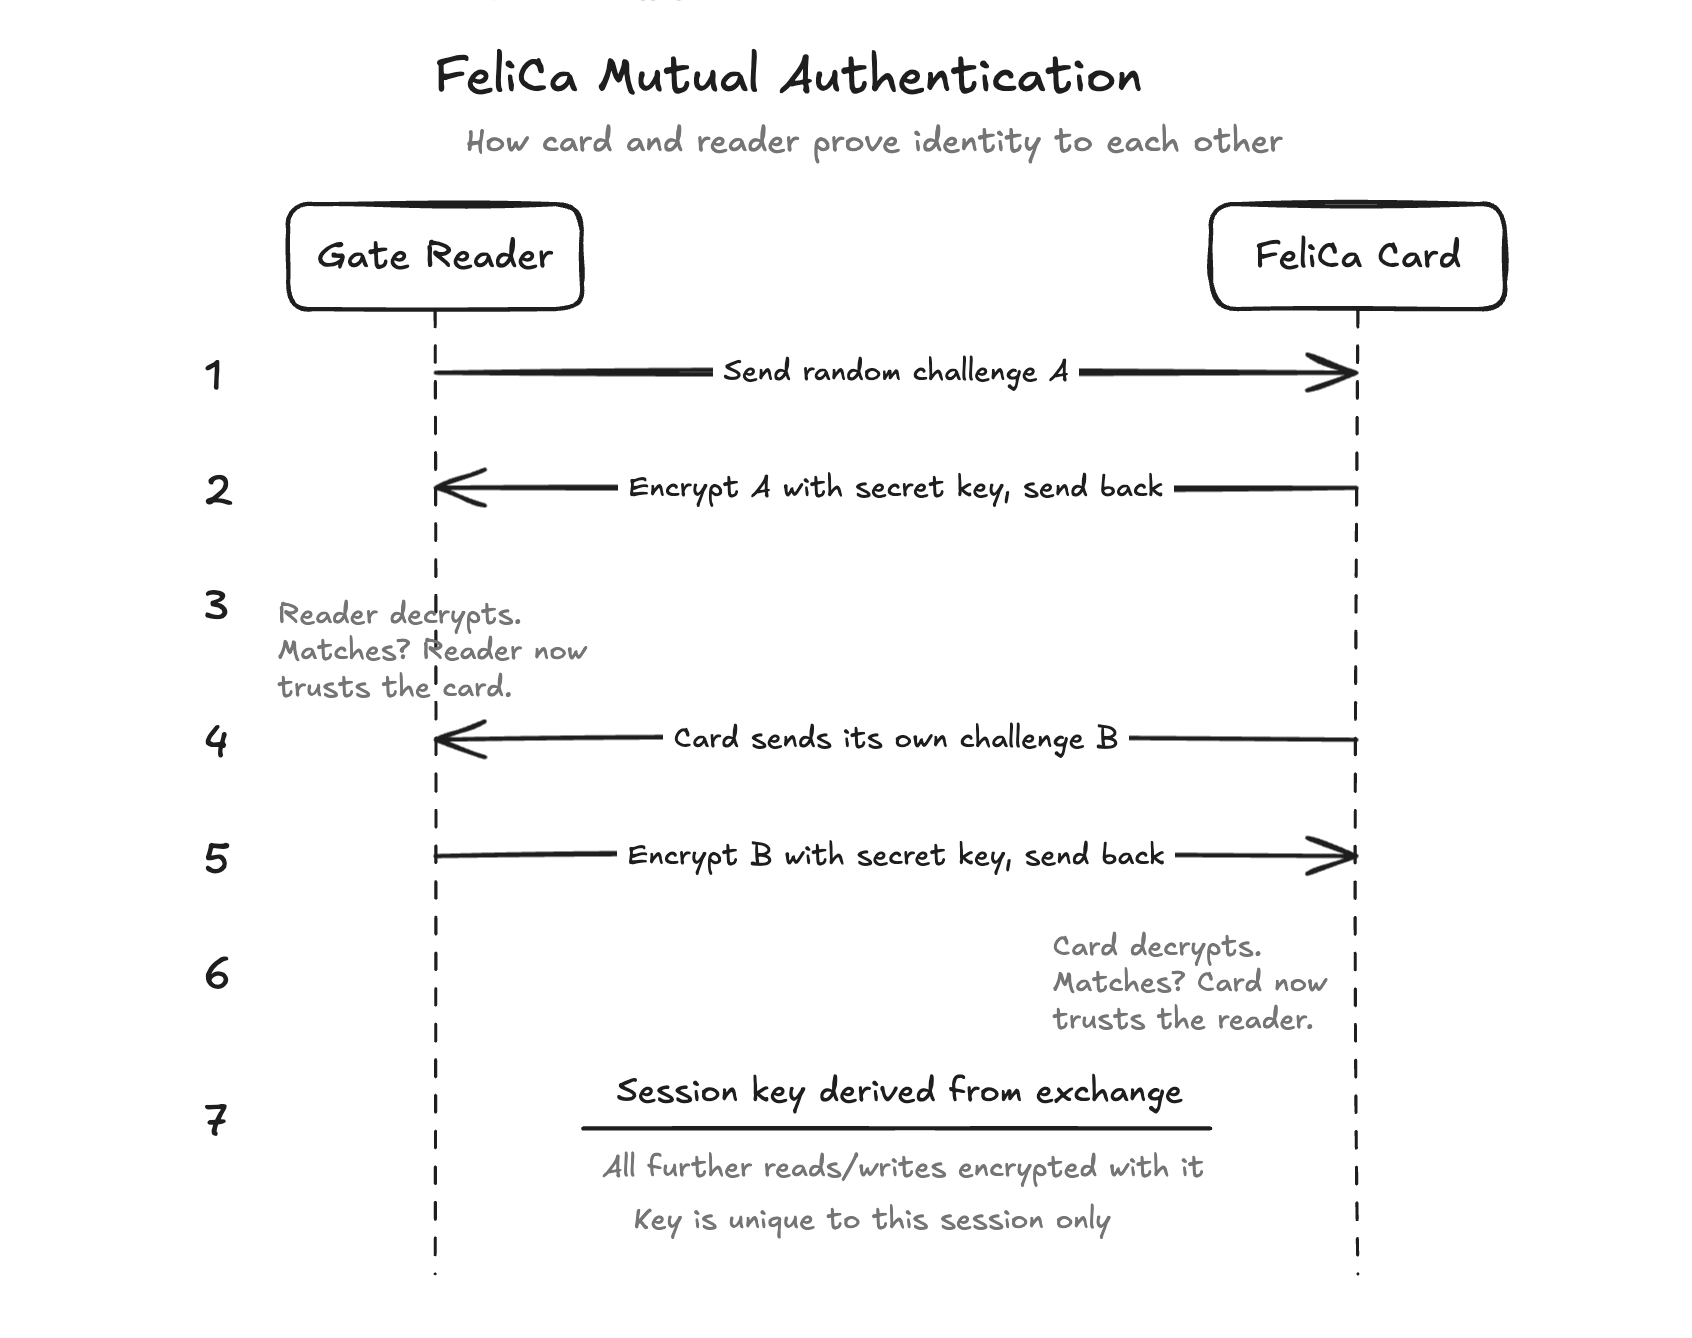
\includegraphics[width=0.85\textwidth]{images/felica-mutual-authentication.png}
    \caption{FeliCa mutual authentication flow between the gate reader and the contactless card. A new encryption key is derived for each session, making captured data useless for future transactions.}
    \label{fig:felica-auth}
\end{figure}

The way mutual authentication works is basically a challenge-response protocol. The reader generates a random number and sends it to the card as a challenge. The card takes that number, encrypts it with the secret key that is stored inside the chip, and sends the encrypted result back. The reader already knows the key too, so it can check if the response is correct. If it is, the reader knows it is talking to a legitimate card and not a fake one. Then the process goes the other way around: the card sends its own random challenge to the reader, the reader encrypts it with the same key, and the card checks the response. Only after both sides have verified each other does the actual balance read and write happen. At the end of this exchange, both sides derive a session key that is used to encrypt everything that follows. This session key is unique to this one transaction and will never be reused.

This design also makes card cloning very hard to pull off. The secret key lives inside the chip's secure memory and it never leaves it. You cannot read it out, not even if you physically open the card. So even if someone has a reader and captures all the radio signals during a transaction, the encrypted responses they capture are useless for next time because the challenges will be different. To fake a valid response, an attacker would need the actual secret key, and there is no way to get it from the captured data alone. What about physical attacks, like putting the chip under a microscope and probing the circuits, or doing power analysis where you measure the chip's electricity consumption to try to figure out the key? That is exactly what the EAL6+ certification covers. To get that certification level, the chip has to be tested against these kinds of hardware attacks and prove it can resist them.

Octopus in Hong Kong follows a similar model but expanded the use case beyond transit. Launched in September 1997, it was actually the first contactless smart card system in the world to adopt Sony's FeliCa technology~\cite{SonyOctopus}, four years before Suica. What started as a pure transit card evolved into a general-purpose stored-value card accepted at convenience stores, restaurants, parking garages, and even vending machines. By the early 2000s, it had over 11 million cards in circulation in a city of 7 million people, which gives you an idea of how widely adopted it became. The interesting thing about Octopus from our perspective is that it demonstrated that a closed-loop, card-stored-balance system could scale beyond its original domain while maintaining fast transaction times.

Now, what can we learn from these systems for our festival payment architecture? The first lesson is that speed matters a lot. Transit systems proved that sub-second transactions are not just nice to have, they are a hard requirement when you are processing large volumes of people who do not want to wait. At a festival, the same principle applies: nobody wants to stand in line for two minutes waiting for a payment to go through when they just want a beer.

The second lesson is about where the balance lives. Transit cards store the balance on the card chip, which is what makes offline operation possible. In a festival context, NFC bracelets can work in a similar way: the balance is written directly to the chip on the bracelet, and the vendor terminal reads and updates it locally, just like a Suica gate does with a FeliCa card. This means transactions can happen even without network connectivity. However, in our system we also support a smartphone app as an alternative to bracelets. With a phone, we cannot write balances directly to the NFC chip the way you can with a bracelet or a transit card. So for the app-based flow, the authoritative balance lives on the server, and during offline periods, vendor terminals work with cached snapshots of recent balances. This dual approach, bracelets with on-chip balances and phones with server-side balances, introduces its own set of challenges, which we will discuss in detail in Chapter~\ref{chap:architecture}.

The third lesson is about the limitations of the transit model. Transit systems operate in a very controlled environment: the terminals are fixed, maintained by professionals, connected to a private network, and the usage patterns are more or less predictable. A festival is a completely different story. Vendor terminals are mobile devices carried by staff who may not be very technical, the network is a temporary Wi-Fi setup in a field, and usage spikes happen unpredictably during meal breaks or between performances. So while transit systems show that offline closed-loop payments can work, their specific solutions do not transfer directly to our context.

\subsection{Festival Payment Systems}
\label{subsec:campus-cards}

Over the past decade, a whole industry has grown up around providing cashless payment solutions for festivals and events. Companies like Tappit, Intellitix, Weezevent, and Glownet have deployed their systems at hundreds of events worldwide. The typical setup works like this: attendees receive an RFID wristband when they enter the festival. They load credits onto the wristband using cash top-up stations or an online portal before the event. At each vendor point, there is a handheld terminal that reads the wristband, deducts the purchase amount, and writes the new balance back to the chip. It is essentially the same model as transit cards, adapted for the festival context.

These systems have proven that cashless festivals are commercially viable. As mentioned in Chapter~\ref{chap:introduction}, Tappit reports that RFID systems reduce transaction times by up to 80 percent compared to cash and increase average spending by about 22 percent~\cite{Tappit2024}. The speed improvement comes from eliminating the need to count cash and make change. The spending increase is attributed to the psychological effect of not physically handing over money, which is consistent with the broader academic literature on cashless payment behavior~\cite{Schomburgk2024}.

However, there are some significant limitations to the RFID wristband approach that motivated us to explore a different path. First, the RFID chips used in most festival wristbands have very limited storage and processing capability. They can store a balance and maybe a transaction counter, but they cannot run complex logic. This means that all the intelligence has to be in the terminal, and the terminal needs to handle things like transaction validation, balance updates, and security checks. If the terminal loses connectivity to the backend and its local cache is stale or incomplete, it has a problem.

Second, and this is the bigger issue, many of these RFID systems rely on MIFARE Classic chips, which have well-documented security vulnerabilities. Garcia et al.~\cite{Garcia2008} demonstrated practical attacks against MIFARE Classic's proprietary CRYPTO1 cipher, showing that the encryption could be broken and the card contents cloned or modified. For a payment system, this is a serious problem because it means that a sufficiently motivated attacker could tamper with their balance. More modern chips like MIFARE DESFire have addressed these vulnerabilities, but they are more expensive, and many festival deployments still use the older technology to keep costs down.

Third, the architectures of these commercial systems are proprietary and essentially undocumented. There is no published academic analysis of how Tappit or Intellitix handle offline operation, conflict resolution, or balance reconciliation. This makes it hard to learn from their design decisions or to identify best practices. All we have are the occasional failure reports, like the Download Festival incident mentioned in Chapter~\ref{chap:introduction}, which tell us what went wrong but not how things were supposed to work.

Since there is not a lot of published research on how these systems work in practice, we talked to people who were involved in deploying payment infrastructure at Untold, one of the largest music festivals in Romania. From those conversations we learned that the typical approach is to deploy a local network on-site and bring dedicated servers to the venue, so that the core payment logic runs locally and does not depend on a remote cloud. Even with this setup though, the network is still unreliable enough that top-up operations can take two to four hours to synchronize across all terminals when the Wi-Fi coverage gets bad. This is a real problem for attendees who just loaded money and want to spend it immediately but the vendor terminal does not know about it yet. It shows that maintaining reliable Wi-Fi coverage is not just something nice to have, it is a core infrastructure requirement for any festival payment system. We discuss how our architecture handles these synchronization delays in Chapter~\ref{chap:architecture}.

Given these trade-offs, there are two main directions we could take. One option is to stick with the RFID wristband model and use NFC bracelets with on-chip balances, which gives us the advantage of fully offline transactions like transit cards but limits what we can do on the user side. The other option is to go with a smartphone app as the consumer device, where the balance lives on the server and payments happen via QR codes or NFC between the phone and the vendor terminal. A phone-based approach gives more flexibility for things like showing transaction history, doing top-ups from the app, and pushing notifications, but it means we depend more on the network since the balance is not stored locally on a chip. There is also a middle ground where we support both. We explore these options further in Chapter~\ref{chap:architecture}.

\subsection{EMV and Offline Authorization}
\label{subsec:emv}

The EMV standard, named after its original creators Europay, Mastercard, and Visa, is the technology behind the chip cards that most people carry in their wallets. While EMV is an open-loop standard designed for the global payment network, it includes a mechanism for offline transaction authorization that is worth understanding because it addresses a similar problem to ours: how do you authorize a payment when you cannot reach the authorization server?

The way EMV offline authorization works is through a set of risk parameters stored on the card chip. The card knows its own balance limits, the maximum amount for a single offline transaction, the maximum number of offline transactions allowed before the card must go online, and the total cumulative amount that can be spent offline. When a merchant terminal cannot reach the bank's authorization server, it can still approve transactions by checking these parameters locally. If the transaction falls within the allowed limits, it gets approved offline. If it exceeds them, the terminal declines the transaction or forces an online authorization attempt.

This is a clever approach because it distributes the risk. The card issuer decides how much offline risk they are willing to accept for each cardholder, and those limits are baked into the card at the time of issuance. A premium cardholder might have higher offline limits than a basic cardholder. The merchant also has some say in this: their terminal can have its own floor limit below which it will always accept transactions without going online.

However, there is a well-known problem with EMV offline authorization: the system trusts the card to honestly report its own state. Murdoch et al.~\cite{Murdoch2010} demonstrated a man-in-the-middle attack on the EMV protocol where a device placed between the card and the terminal could trick the terminal into believing that a PIN had been correctly verified when it had not. While this specific attack targets the PIN verification rather than the offline balance logic, it illustrates a broader point: any system where the authorization decision depends on data stored on a device in the user's possession is vulnerable to tampering if the security of that device is compromised.

For our system, the EMV offline model offers both inspiration and a warning. On the inspiration side, the idea of using spending limits to control offline risk is directly applicable. We implement something similar: during offline periods, vendor terminals enforce a maximum transaction amount and a maximum total offline spend per consumer, which limits the potential damage from double-spending or stale balance snapshots. On the warning side, the EMV experience shows that offline authorization always involves a trade-off between availability and security. The more you allow offline, the more risk you accept. Our system handles this by keeping offline periods as short as possible and treating offline mode as a temporary fallback rather than a primary operating mode.

\section{Offline-First Architecture Patterns}
\label{sec:offline-first}

When you build a system that needs to work without a network connection, you are basically deciding where on a spectrum your application sits. On one end you have fully online systems, where every operation needs a round-trip to a server and nothing works without internet. On the other end you have fully offline systems, like the FeliCa transit cards we discussed earlier, where everything happens locally and the network is only used for background synchronization. Most real-world applications fall somewhere in between.

For our festival payment system, we need to be somewhere in the middle of this spectrum. The system should work online by default, because that gives us the strongest guarantees about balance correctness and transaction ordering. But when the network goes down, and at a festival it will go down, the system needs to keep processing payments using whatever data it has cached locally. This means we need architectural patterns that support both modes of operation and can switch between them without losing data or creating inconsistencies that cannot be resolved later.

In this section we look at four architectural patterns that are relevant to this problem. Each one addresses a different aspect of building systems that can work without constant connectivity.

\subsection{Local-First Software}
\label{subsec:local-first}

The term ``local-first software'' was introduced by Kleppmann et al.~\cite{Kleppmann2019} in a 2019 paper that argued for a different way of thinking about where data lives in an application. The basic idea is that the primary copy of the data should be on the user's local device, not on a remote server. The cloud still exists, but its role is to sync data between devices rather than to be the single source of truth. If the server goes down, or the network disappears, the application keeps working because the data is right there on the device.

Kleppmann and his co-authors defined seven ideals for local-first software: no spinners (the app should be fast because it reads from local storage), the user's work should be available on multiple devices, the network should be optional, collaboration should be seamless, the data should be accessible for a long time (not locked behind a service that might shut down), security and privacy should be built in, and the user should have full ownership and control over their data.

Now, our festival payment system does not fit neatly into the local-first model, and there is a good reason for that. In a collaborative document editor, if two people edit the same paragraph and the results get merged a bit awkwardly, that is annoying but not catastrophic. In a payment system, if two terminals both think a user has 50 euros and each one authorizes a 40 euro purchase, you have just lost 30 euros. Money is a conserved quantity. You cannot merge two versions of a balance the way you merge two versions of a text document.

That said, some of the local-first principles are directly useful for us. The idea of keeping a local copy of the data so the app does not freeze when the network drops is exactly what our vendor terminals need to do. The difference is that in our case, the local copy is a read cache with limited write authority, not the primary copy. The server remains the source of truth, and offline transactions are treated as provisional until they get confirmed by the server. This is a weaker version of local-first, but it is the right trade-off for a system where financial correctness matters more than collaboration flexibility.

\subsection{Conflict-Free Replicated Data Types (CRDTs)}
\label{subsec:crdts}

CRDTs, or Conflict-Free Replicated Data Types, are data structures specifically designed for systems where multiple nodes can modify the same data independently, without coordinating with each other, and still end up in a consistent state. They were formalized by Shapiro et al.~\cite{Shapiro2011} in 2011, and the key property that makes them work is that all operations on the data structure are designed to be commutative, associative, and idempotent. What this means in practice is that it does not matter what order the updates arrive in, or if some updates arrive more than once. The result will always be the same.

The simplest example is a G-Counter (grow-only counter). Imagine you have five terminals at a festival, and each one counts how many transactions it has processed. Each terminal only increments its own counter. When they sync, you just take the maximum value for each terminal's counter and sum them up. No conflicts possible. A PN-Counter extends this idea by having two G-Counters, one for increments and one for decrements, and the actual value is the difference between the two.

This sounds like it could work for tracking balances, but there is a catch. A balance is not just a counter that goes up and down freely. Money is conserved: you cannot spend more than you have. CRDTs are great at ensuring convergence (everyone ends up with the same value), but they do not enforce invariants like ``the balance must not go below zero.'' If two terminals independently authorize purchases against the same balance while offline, a naive CRDT approach would let both go through, even if the total exceeds the available balance. You would only discover the overspend after synchronization.

Kleppmann~\cite{Kleppmann2017json} explored this limitation in the context of JSON CRDTs and noted that while CRDTs guarantee convergence, they do not guarantee that the converged state is one that any individual node would have accepted. For payment systems, this is a real problem. We cannot just let every offline transaction go through and hope the math works out later.

So for a payment system, pure CRDTs are not enough on their own. You need something extra on top to deal with the fact that balances have constraints. There are a few ways to handle this. One option is to record offline transactions as events and have the server replay and validate them when connectivity returns, rejecting any that would overdraw the balance. Another option is to pre-allocate spending limits per terminal so that each terminal can only authorize up to a fixed amount while offline, which reduces the chance of overspending in the first place. A third option is some combination of the two. We explore these trade-offs further in Chapter~\ref{chap:architecture}.

\subsection{Event Sourcing and CQRS}
\label{subsec:event-sourcing}

Event sourcing is a pattern where instead of storing the current state of an object (like ``balance = 47.50''), you store the entire sequence of events that led to that state (``topped up 50.00, bought beer for 2.50''). The current state can always be reconstructed by replaying the events from the beginning. Fowler~\cite{Fowler2005} describes event sourcing as a way to ``ensure that all changes to application state are stored as a sequence of events,'' and one of the main benefits is that you get a complete audit trail for free.

This pattern fits really well with offline payment processing. When a vendor terminal goes offline, it cannot update the central database directly. But it can keep recording events locally: ``user X paid 5.00 for item Y at timestamp Z.'' Each event is self-contained and immutable. When the terminal reconnects, it uploads its event log to the server, and the server can process these events in order to update the authoritative state. If there is a conflict (say, the user ran out of money between two offline purchases), the server can detect it during replay and handle it according to whatever policy the operator has defined.

CQRS, which stands for Command Query Responsibility Segregation, is a related pattern that is often used together with event sourcing. The idea, as described by Young~\cite{Young2010}, is to separate the write side of the system (commands that modify state) from the read side (queries that return data). In a traditional system, the same data model handles both reads and writes. In CQRS, you have one model optimized for processing writes (accepting payment events) and another model optimized for fast reads (showing the current balance on a screen).

For our system, this separation is useful because the write side and the read side have very different requirements. On the write side, we need strong ordering guarantees and conflict detection. On the read side, vendor terminals need to quickly look up a user's balance to decide whether to authorize a payment, and this lookup needs to work even when the terminal is offline. By separating these concerns, we can have the read model work from a local cache while the write model queues events for later synchronization, without the two getting in each other's way.

\subsection{Edge Computing}
\label{subsec:edge-computing}

Edge computing is the idea of moving computation closer to where the data is generated, instead of sending everything to a central server or cloud for processing. Shi et al.~\cite{Shi2016} describe it as ``pushing the frontier of computing applications, data, and services away from centralized nodes to the logical extremes of a network.'' In practice, this means doing as much work as possible on the device that is closest to the user, and only involving the cloud when necessary.

In the context of our festival payment system, the vendor terminals are the edge nodes. Each terminal runs a local instance of the payment logic: it can read a user's balance from its local cache, validate a transaction against the cached data, record the transaction as an event, and update its local view of the balance. All of this happens on the terminal itself without any network communication. The cloud server (or the on-site local server, as we discussed in the context of the Untold festival) acts as the central coordinator that collects events from all the edge nodes, resolves conflicts, and pushes updated state back out.

This works well for festival environments because the network is the weakest link in the whole system. The less you depend on it for individual transactions, the better. If the terminal can handle a payment entirely on its own, then a network outage does not mean a payment outage. It just means that the synchronization of data gets delayed. The trade-off, of course, is that edge nodes are working with potentially stale data. A terminal that has been offline for 30 minutes might not know about a top-up that happened 20 minutes ago. How we handle this staleness, and what limits we put on edge-processed transactions to manage the risk, is something we cover in detail in Chapter~\ref{chap:architecture}.

\section{Conflict Resolution in Distributed Systems}
\label{sec:conflict-resolution}

When multiple vendor terminals at a festival are processing payments independently, without being able to talk to each other or to a central server, they are going to end up with different views of the world. Terminal A might think a user has 50 euros because it processed a top-up, while Terminal B still shows the old balance of 20 euros because it has not received the update yet. If both terminals authorize purchases during this window, the system will have conflicting records that need to be sorted out once everyone reconnects.

This is not a new problem. Distributed systems have been dealing with conflicting state for decades, and there is a solid body of theory and practice around how to handle it. In this section we go through the main concepts that are relevant to our case: what trade-offs are fundamental and cannot be avoided, how systems achieve consistency without requiring all nodes to agree in real-time, how to figure out the order of events when there is no shared clock, and how to let nodes work independently with the plan of fixing things up later.

\subsection{The CAP Theorem}
\label{subsec:cap-theorem}

In 2000, Eric Brewer presented a conjecture at the ACM Symposium on Principles of Distributed Computing that would become one of the most cited results in distributed systems. The conjecture, which Gilbert and Lynch~\cite{Gilbert2002} formally proved in 2002, says that a distributed system can only guarantee two out of three properties at the same time: Consistency (every node sees the same data at the same time), Availability (every request to a non-failing node gets a response), and Partition Tolerance (the system keeps working even when the network between nodes is broken).

The important word here is ``partition tolerance.'' In a festival environment, network partitions are not an edge case, they are a regular occurrence. When the Wi-Fi drops between two parts of the venue, the vendor terminals on each side are partitioned from each other and from the server. At that point, according to CAP, we have to choose: do we want consistency or availability?

If we choose consistency, then when a terminal cannot reach the server to verify a balance, it should refuse the transaction. The data stays consistent, but the system is unavailable and the attendee cannot buy anything. If we choose availability, the terminal goes ahead and authorizes the payment based on its local cache, even though it cannot be sure the data is up to date. The payment goes through, the attendee is happy, but we might end up with inconsistencies that have to be fixed later.

For a festival payment system, refusing transactions because the network is down is not really an option. Nobody is going to accept a system that stops working every time the Wi-Fi gets flaky, which at a festival is all the time. So during network partitions, our system leans toward availability. Transactions keep going through, and consistency is restored after the partition heals. This is not a unique choice. Many real-world systems choose availability during partitions and then run a reconciliation process afterward. That is essentially what we are doing.

\subsection{Eventual Consistency}
\label{subsec:eventual-consistency}

If we are giving up strong consistency during network partitions, the question becomes: what kind of consistency can we actually promise? The answer, for most distributed systems that prioritize availability, is eventual consistency. Vogels~\cite{Vogels2009} defines it simply: if no new updates are made to a piece of data, then eventually all replicas will converge to the same value.

The word ``eventually'' is doing a lot of work in that definition. It does not say when the replicas will agree, just that they will at some point. In practice, this usually happens pretty fast once connectivity is restored. But during the partition, different nodes can have different views of the data, and that is considered acceptable.

The most famous real-world example of eventual consistency is Amazon's Dynamo, described by DeCandia et al.~\cite{DeCandia2007}. Dynamo is a key-value store that Amazon built for their shopping cart and other services that need to be available all the time, even during failures. Dynamo allows writes to happen on any node, even if that node cannot reach the others. When the partition heals, Dynamo uses application-specific logic to merge conflicting versions.

For our system, eventual consistency means the following: while terminals are offline, they work with their local data and record all transactions locally. When they reconnect, they send their transaction logs to the server. The server processes everything, figures out the correct state of each balance, and pushes the updated data back to all terminals. At that point, everyone is consistent again. The window during which terminals might have stale or conflicting data is the offline period, and the goal of the architecture is to make this window as short as possible and to limit the damage that can happen during it (for example, by capping how much a terminal can authorize while offline).

\subsection{Transaction Ordering and Why Timestamps Are Enough}
\label{subsec:transaction-ordering}

One of the classic problems in distributed systems is figuring out the order in which things happened across different nodes. The standard solutions from the literature are logical clocks and vector clocks, which use counters instead of real time to establish ordering. These are necessary in systems like high-frequency trading platforms, where events happen microseconds apart on different machines and physical clock drift is larger than the interval between events.

However, for a festival payment system, the situation is fundamentally different. Transactions happen at human speed. A person walks to a vendor, waits in line, orders something, taps their wristband. The gap between one transaction and the next, even for the same user, is measured in minutes, not microseconds. Even cheap NTP synchronization keeps clocks within a few hundred milliseconds of each other, and that kind of drift is completely irrelevant when the events we care about are minutes apart.

This means that plain wall-clock timestamps, recorded by each vendor terminal at the moment of the transaction, give us unambiguous ordering in practice. There is no realistic scenario where two transactions from the same user happen so close together that clock drift changes the order. The physical constraint of the wristband model reinforces this: a user can only be at one vendor at a time, so transactions from the same user are naturally serialized by their physical presence.

The practical advantage of using timestamps over vector clocks is significant. With timestamps, vendor terminals do not need to communicate with each other at all during offline periods. Each terminal just records its local time with each transaction. When the network comes back, everyone pushes their logs to the server, the server sorts by timestamp, and we are done. There is no vector state to maintain, no counter synchronization between devices, and no extra complexity in the protocol. For a system that needs to work reliably in a festival environment where connectivity is unreliable, this simplicity is a real advantage.


\chapter{System Architecture}
\label{chap:architecture}

This chapter goes through the architecture of the closed-loop payment system. We start with the big picture, explain why we chose this approach over the alternatives, and then go into each component one by one. The whole idea behind the design is to keep things simple: one server, one app that works for everyone, and strive to have always network support. If network however will go down the balance will be always cached on the bracelet and used as a deciding factor if the payment will be approved or not. The system should be easy to deploy, easy to understand, and tough enough to handle what actually happens at a festival.

\section{High-level overview}
\label{sec:high-level-overview}

Most existing festival payment systems need a technical team to physically go to the venue, set up local servers, deploy a private network, and babysit the infrastructure for the entire duration of the event. As we discussed in Section~\ref{subsec:campus-cards}, the standard approach at festivals like Untold involves bringing dedicated servers on-site so that the payment logic runs locally. This makes sense when the balance lives on a remote server and every transaction needs a network round-trip to authorize. In that model, if the connection between the venue and the cloud drops, nobody can pay for anything, so you bring the server to the venue to avoid that dependency.

Our system takes a different path. As mentioned, we strive to always have reliable internet access using Starlink as the primary uplink, paired with a redundant network topology that keeps terminals talking to the server even when individual links degrade. The bracelet-as-cache fallback exists for the residual edge cases, but the goal is to never need it.

This means there is no need to deploy anything at the festival venue. No local servers, no private network infrastructure, no IT team on-site. The organizer creates an event through the admin dashboard, configures the parameters, approves the vendors, and distributes the wristbands. The vendors download the app, get whitelisted, and they are ready to accept payments. The server runs in the cloud, the same way it runs for every other festival on the platform. Nothing changes in the deployment.

The system has four main components: a backend server, a mobile application for attendees and vendors, a web-based admin dashboard, and NFC wristbands that carry the actual token balance for each attendee. The server is a single, multi-tenant service that manages all festivals from one deployment. There is no need to spin up a separate server or database for each event. An admin creates an event, configures it, and the system handles the rest. The mobile app is what attendees and vendors interact with: attendees see their balance and history, and vendors use it as a soft point-of-sale terminal. Admins manage the event through a separate web dashboard that works in any browser. The wristband is where the balance actually lives during the event.

Figure~\ref{fig:system-architecture} shows the high-level architecture of the system. The thing to notice is the NFC connection between the Vendor POS and the wristband at the bottom: that is the actual payment path, and it does not go through the server. Everything above that (the load balancer, the server instances, the database) is for management, reporting, and synchronization, not for processing individual payments.

\begin{figure}[ht]
	\centering
	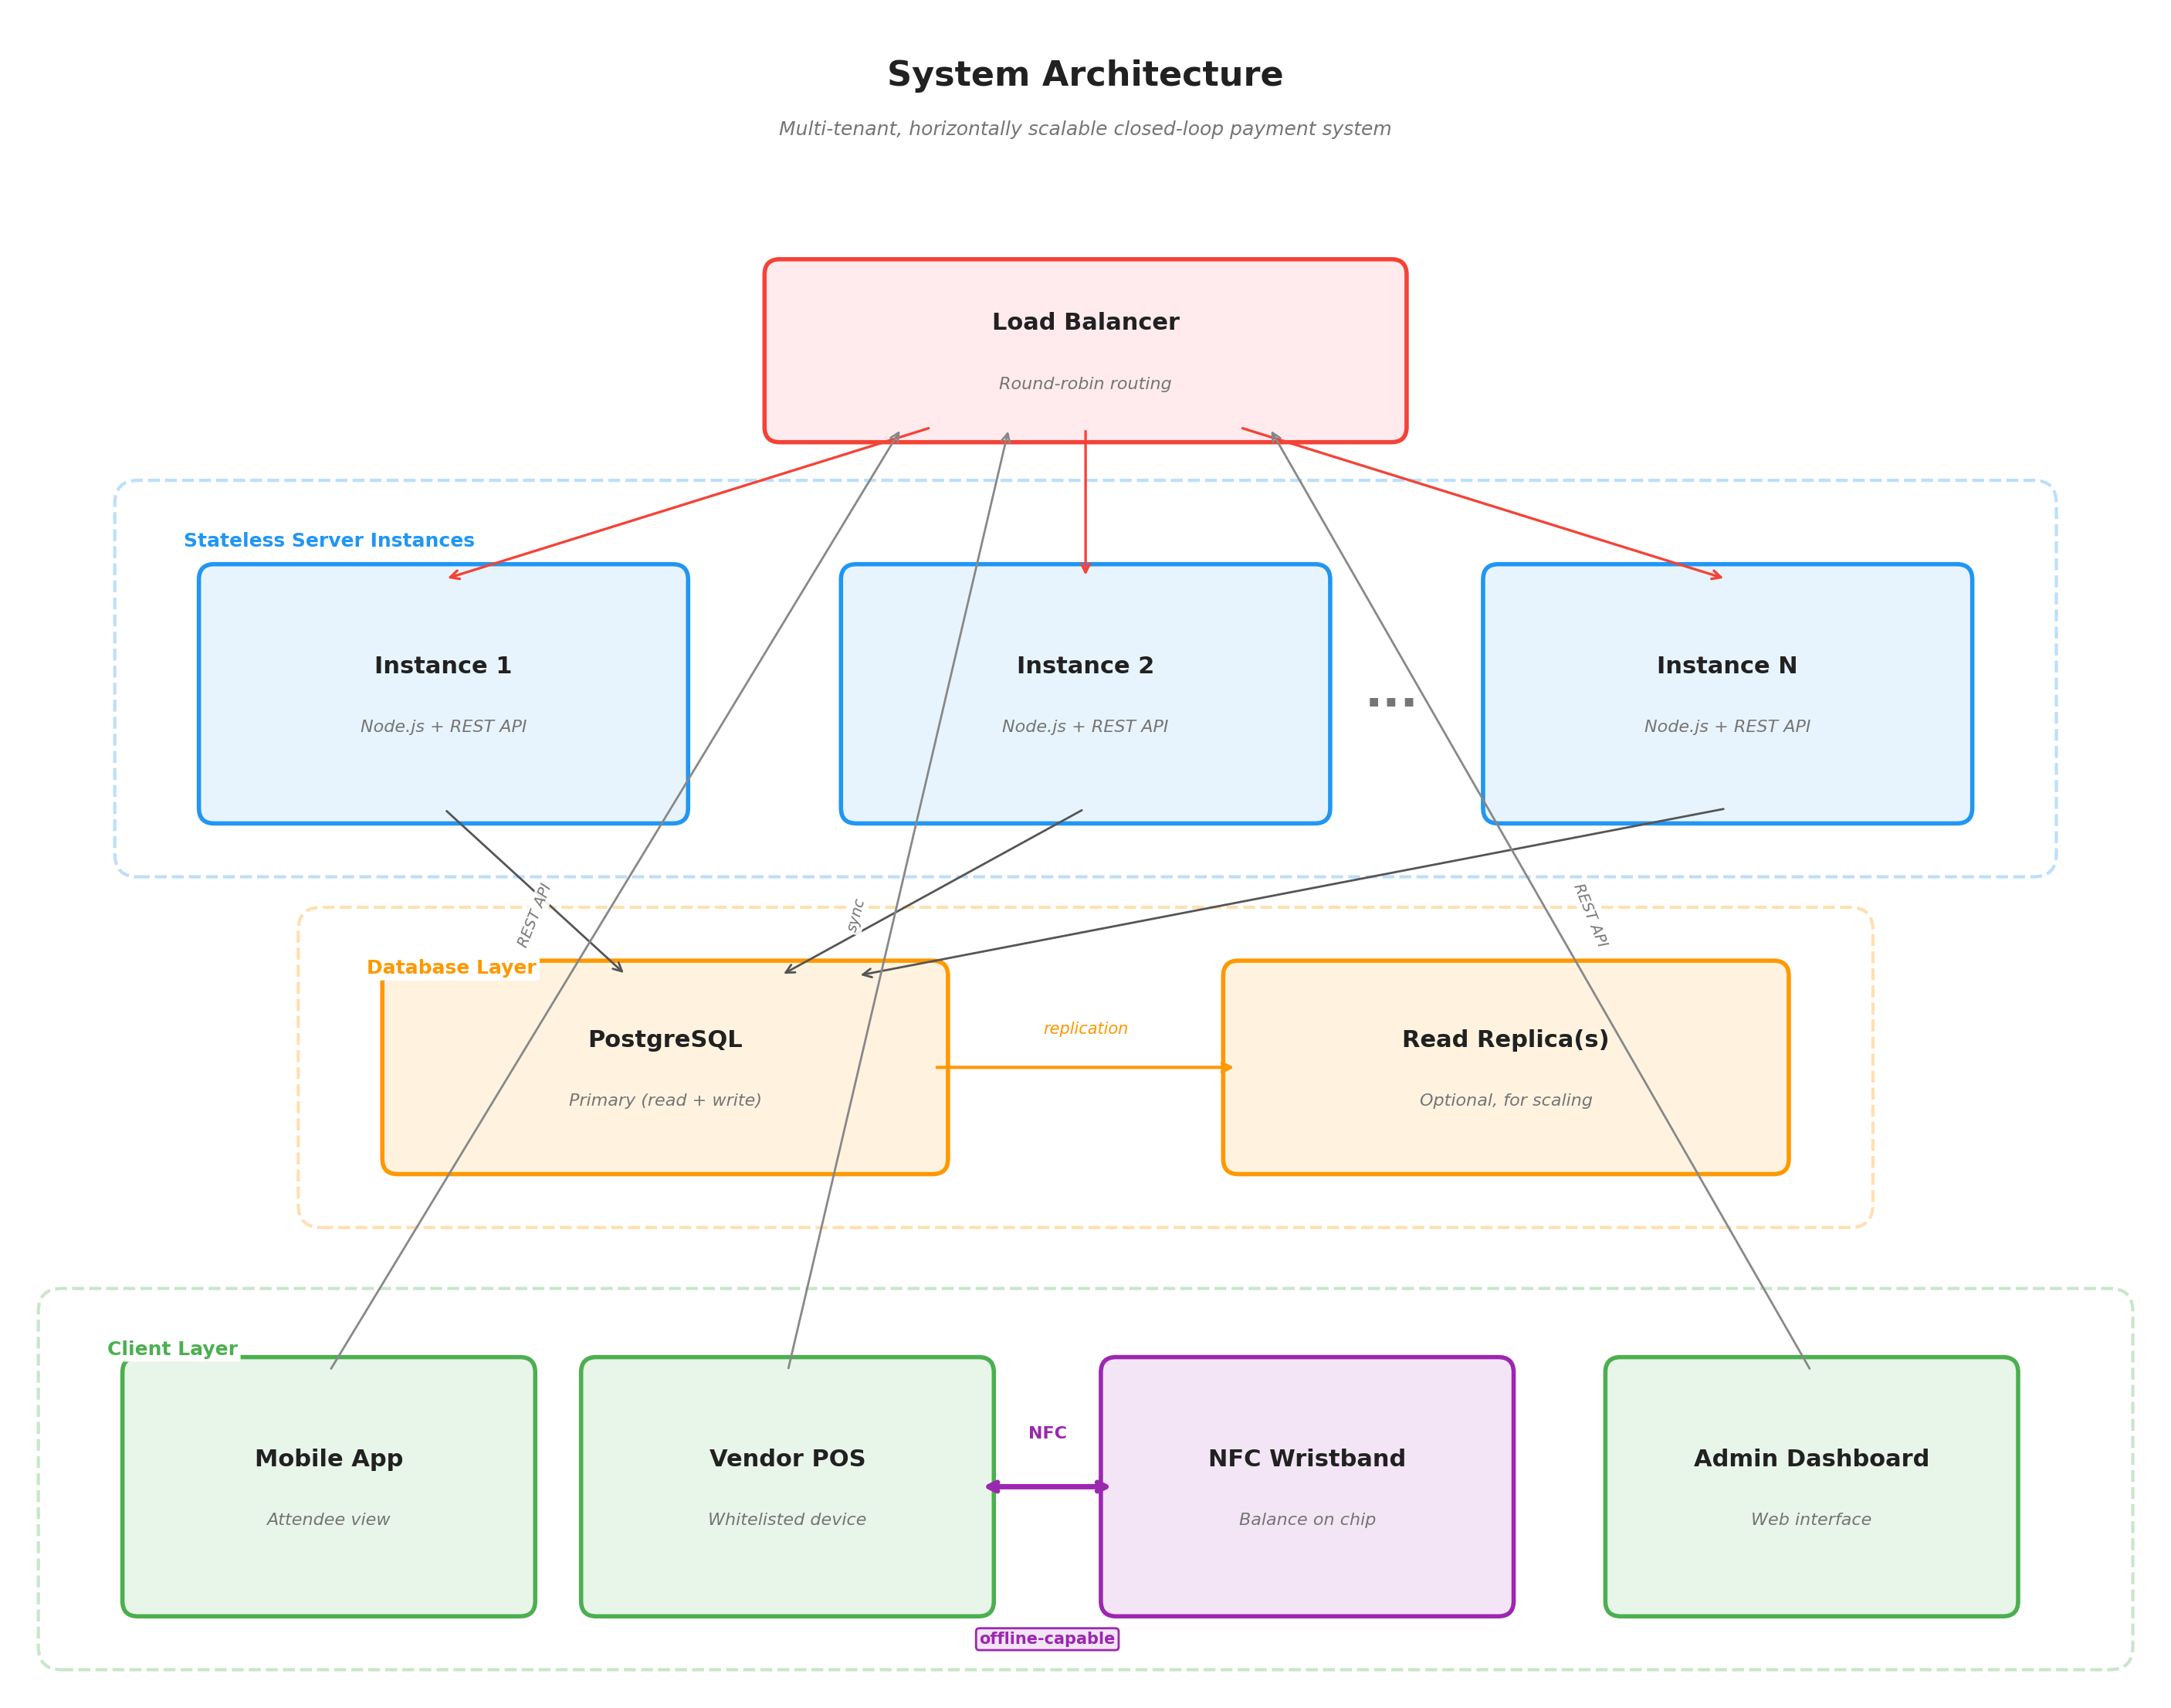
\includegraphics[width=0.95\textwidth]{images/system-architecture.png}
	\caption{High-level system architecture. Payments happen directly between the vendor device and the NFC wristband without server involvement. The backend handles event management, top-ups, and transaction log synchronization. Server instances are stateless and horizontally scalable behind a load balancer.}
	\label{fig:system-architecture}
\end{figure}

\section{Why this architecture}
\label{sec:why-architecture}

Before settling on this design, we considered a few different approaches and went through the techniques and patterns discussed in Chapter~\ref{chap:background} to figure out which ones are actually useful in our context and which ones would just add complexity for no real benefit. The choice of where the balance lives is really the decision that shapes everything else, so it is worth comparing the options side by side and explaining what we took from the literature and what we left behind.

\subsection{Architecture comparison}
\label{subsec:architecture-comparison}

\textbf{Option A: Server-side balance, online-only.} The wristband (or QR code, or whatever the attendee carries) is just an identifier. Every time a vendor scans it, the terminal sends a request to the server, which checks the balance, deducts the amount, and sends back a confirmation. This is the simplest model to reason about because the server is always the single source of truth. The problem is obvious: if the network goes down, payments stop completely. For a regular retail store this is fine because they have stable internet. For a festival with 50,000 people in a field, it is not.

\textbf{Option B: Server-side balance with local cache.} Same as Option A, but vendor terminals keep a cached copy of recent balances. When the network drops, they fall back to the cache. This sounds reasonable until you think about what happens when two vendors both have a cached balance of 50 tokens for the same user. Vendor A deducts 40, Vendor B deducts 40, and now the user has spent 80 tokens out of 50, caching the balance on the vendors devices still does not achieve anything if the cache is not shared between them.

\textbf{Option C: Balance cached on the wristband, server as source of truth.} The NFC chip on the wristband caches the user's balance, but the server remains the canonical record. In normal operation, vendors authorize against the server, which debits the balance and writes the updated value back to the chip. If connectivity drops, terminals fall back to the cached balance on the chip: they read it, verify funds, debit the chip, and queue the transaction locally for replay once the network returns. The user can only be in one place at a time, so the wristband naturally serializes transactions during offline periods, and a monotonic counter on the chip lets the server detect and apply queued debits in order without double-counting. This is the same principle that makes transit card systems like Suica and Octopus work: the card is fast and offline-capable, but the back office is always the authoritative ledger.

Table~\ref{tab:architecture-comparison} summarizes the comparison.

\begin{table}[ht]
	\centering
	\begin{tabular}{|l|c|c|c|}
		\hline
		\textbf{Criteria} & \textbf{A: Online-only} & \textbf{B: Cached} & \textbf{C: On wristband} \\
		\hline
		Works offline & No & Partially & Yes \\
		\hline
		Double-spend risk & None & High offline & None \\
		\hline
		Server dependency & Every tx & Every tx + cache & Sync only \\
		\hline
		On-site infrastructure & Required & Required & Not needed \\
		\hline
		Physical tamper risk & None & None & Needs secure chip \\
		\hline
		Complexity & Low & High & Medium \\
		\hline
	\end{tabular}
	\caption{Comparison of the three architectural approaches for storing the user balance.}
	\label{tab:architecture-comparison}
\end{table}

\subsection{What we learned from existing systems}
\label{subsec:lessons-existing}

In Chapter~\ref{chap:background} we looked at transit cards, commercial festival payment systems, and the EMV offline authorization model. Each one influenced our design in different ways.

Transit card systems like Suica and Octopus (Section~\ref{subsec:transit-cards}) are basically the proof that Option C works at scale. Suica processes millions of transactions per day with sub-second speed, all because the balance lives on the FeliCa chip and the gate does not need to call any server. Our wristband model takes the same core idea: the balance is on the chip, the terminal reads it, deducts, and writes back. The difference is that Suica runs on fixed gates maintained by professionals in train stations with dedicated private networks, while we run on random phones carried by festival vendors in a field. So the principle transfers, but the implementation details are quite different. We also borrowed the security model from FeliCa, specifically the mutual authentication between the chip and the reader, which we implement using MIFARE DESFire's AES-128 protocol instead of FeliCa's proprietary encryption. The idea is the same: both sides prove to each other that they are legitimate before any data gets exchanged.

From the commercial festival systems like Tappit and Intellitix (Section~\ref{subsec:campus-cards}), we mainly learned what we do not want to do. These systems require an IT team to go to the venue, set up local servers, deploy a private network, and manage the whole thing for the duration of the event. That works for a company with dedicated operations staff, but it does not work if the goal is a system that a small organizer can deploy by themselves. The conversations we had with people who worked on the Untold deployment confirmed this: even with dedicated on-site infrastructure, top-up synchronization delays of two to four hours were common when the Wi-Fi got bad. Our architecture avoids this entirely because there are no on-site servers to maintain. The wristband handles payments locally, and the cloud server only needs to be reachable for top-ups and sync, which can tolerate delays without blocking the actual payment flow.

The EMV offline authorization model (Section~\ref{subsec:emv}) gave us the idea of using spending limits as a risk control mechanism. EMV cards carry parameters that define how much they can spend offline before they have to go online for authorization. We use a similar concept: the event admin can configure maximum transaction amounts and maximum total offline spend per wristband. This is mostly relevant as a safety net for the edge case where someone does manage to tamper with a wristband, it limits the potential damage. But unlike EMV, where the card self-reports its own state and the terminal has to trust it (which, as Murdoch et al.~\cite{Murdoch2010} showed, is exploitable), our DESFire wristbands authenticate cryptographically before every read and write. The terminal does not take the wristband's word for it, it verifies through the shared AES key.

\subsection{What we took from the architectural patterns}
\label{subsec:lessons-patterns}

In Section~\ref{sec:offline-first} we covered several architectural patterns for offline operation: local-first software, CRDTs, event sourcing with CQRS, and edge computing. Not all of them ended up being useful for our case.

\textbf{Local-first software} (Section~\ref{subsec:local-first}) is a nice philosophy, but as we discussed in Chapter~\ref{chap:background}, it does not fit payment systems well. Kleppmann et al.~\cite{Kleppmann2019} designed it for collaborative applications where merging conflicting edits is annoying but acceptable. With money, you cannot just merge two conflicting balance updates and hope for the best. Our system borrows the basic idea of keeping a local copy of data so the app works without the network, but the server remains the source of truth and offline transactions are treated as provisional. It is a weaker version of local-first, and that is the right call for a system where financial correctness actually matters.

\textbf{CRDTs} (Section~\ref{subsec:crdts}) are an interesting solution for data convergence in distributed systems, but they turned out to be overkill for what we need. CRDTs guarantee that all replicas converge to the same value regardless of the order updates arrive, which sounds great until you realize they cannot enforce constraints like ``the balance must not go below zero.'' In our case, since the balance lives on the wristband, we do not really have a distributed data convergence problem in the first place. The wristband is the single copy of the balance during the event. There is nothing to converge. The server's copy is just a log of what happened, reconstructed from the transaction events that vendor devices upload. So CRDTs would add complexity to solve a problem that our architecture does not have.

\textbf{Event sourcing} (Section~\ref{subsec:event-sourcing}) is the one pattern we actually use directly. Every transaction that happens on a vendor device is recorded as an immutable event with a timestamp, a device ID, a wristband ID, and the amount. When the device is online, these events are sent to the server immediately. When it is offline, they queue up locally and get pushed as a batch when connectivity returns. The server reconstructs the state of each wallet by replaying these events. This gives us a full audit trail of everything that happened, which is important for settlement and for the event organizer to see where the money went. We do not use CQRS in the formal sense (separate read and write models), but in practice the vendor app does maintain a local read cache of recent transactions that is separate from the write queue, which is a similar idea.

\textbf{Edge computing} (Section~\ref{subsec:edge-computing}) shows up in our architecture at two levels. The first and more obvious one is the vendor phones themselves. Each phone runs the payment logic locally: read the wristband, validate the balance, deduct, write back. The cloud server coordinates and collects data, but it is not in the critical path of a payment. We also pushed the state further out than a typical edge setup, all the way to the wristband itself, so the edge node (the phone) does not even need to maintain a local copy of the balance. It reads the authoritative state directly from the chip every time. The second level is the server deployment itself. We deploy on Railway, which lets us pick the region where the container and the database run. So for festivals in Romania or elsewhere in Europe, the backend sits in a European data center with low latency to the vendor devices, instead of routing everything through some server in the US. For the operations that do need the server (top-ups, sync, admin dashboard), this makes a noticeable difference in responsiveness. And if the platform ever expands to other continents, spinning up another region on Railway is just a configuration change, no need to touch the application code.

\textbf{The CAP theorem} (Section~\ref{subsec:cap-theorem}) told us what we already knew intuitively: during a network partition at a festival, we have to choose between consistency and availability, and refusing transactions because the Wi-Fi dropped is not acceptable. Our architecture sidesteps the hardest part of this tradeoff by putting the balance on the wristband. With Option B (server-side balance with cache), you are fully in CAP territory because the cached balances on different terminals can diverge and you get double-spend. With Option C (balance on wristband), the wristband itself acts as a single, physically consistent copy that moves with the user. There is no partition between the balance and the terminal that is reading it, because they are in direct NFC contact. The CAP tradeoff still applies to the synchronization of transaction logs with the server, but there the worst case is delayed reporting, not double-spending, which is a much smaller problem.

So to sum it up: from the existing systems we took the on-chip balance model (transit cards), spending limits as a safety net (EMV), and the lesson that on-site infrastructure should be avoided (festival systems). From the architectural patterns, we took event sourcing for the transaction log and edge computing as the general execution model, but we left behind local-first's strong local ownership model and CRDTs because the wristband balance model makes them unnecessary.

\section{NFC wristbands and offline support}
\label{sec:wristband-offline}

Since the balance lives on the wristband, the offline story becomes much simpler than it would be with a server-side model. This section explains how the wristband interaction works, what happens during offline periods, and how the system reconciles everything once connectivity comes back. We also touch on the security considerations here, because with the balance stored physically on the chip, security is part of the architecture, not something you bolt on afterwards.

\subsection{How a payment works}
\label{subsec:how-payment-works}

The transaction flow between the vendor device and the wristband goes like this:

\begin{enumerate}
	\item The vendor enters the amount (or selects items from a product catalog) on their phone.
	\item The customer taps their wristband against the phone's NFC reader.
	\item The app reads the current balance and transaction counter from the wristband.
	\item The app checks that the balance is sufficient.
	\item The app writes the new (lower) balance and an incremented counter back to the wristband.
	\item Only after a successful write confirmation, the transaction is recorded as completed in the local log.
	\item If the write fails (customer pulled their wrist away too quickly, interference, etc.), the transaction is marked as failed and the vendor is prompted to retry.
\end{enumerate}

This ordering is important. The vendor device never records a successful payment unless the wristband was actually updated. The worst case scenario is that the vendor has to ask the customer to tap again, which is a small inconvenience but not a financial problem.

\subsection{Offline operation}
\label{subsec:offline-operation}

During normal online operation, vendor terminals send each transaction to the server right after it is recorded locally. The server updates its own ledger, which is the authoritative record for reporting, settlement, and auditing.

When the network goes down, vendor terminals keep processing payments exactly as before. The wristband interaction does not change at all. The only difference is that transactions accumulate in the local queue on the vendor device instead of being sent to the server. Once connectivity returns, the device pushes its queued transactions to the server in a batch.

\subsection{Balance reconciliation model}
\label{subsec:balance-reconciliation}

A closed-loop payment system with offline-capable terminals has two writers that can mutate balance state: the server (when users top up) and the chip (when users pay vendors). During a network partition, both can act independently, and the system has to converge on a correct final state once connectivity is restored. This is a well-studied problem in distributed systems, and naive solutions tend to either double-spend, double-credit, or lose money in subtle ways.

Our model relies on a strict separation of concerns between the two writers. The server is the only writer for credits (top-ups, refunds, adjustments). The chip is the only writer for debits (vendor payments). Because the two operation types live in disjoint lanes, no merge conflict is possible: addition and subtraction commute, and each lane has exactly one authoritative source. We require top-ups to be online-only, which keeps the credit lane fully under server control and avoids the entire class of problems that arise when both sides can issue credits independently.

\subsubsection{State and counters}

Each wristband stores four fields: \texttt{balance} (the cached balance in minor units), \texttt{debit\_counter} (a monotonic counter incremented on every chip-side debit), \texttt{credit\_counter\_seen} (the highest server-side credit sequence the chip has acknowledged), and identity fields (\texttt{bracelet\_uid}, \texttt{event\_id}) written at provisioning.

The server maintains per-wallet: \texttt{balance} (the canonical balance), \texttt{credit\_counter} (incremented on every server-side credit), and \texttt{debit\_counter\_seen} (the highest debit counter value the server has reconciled from any terminal).

The two counters are independent monotonic sequences, each with a single writer. The chip owns \texttt{debit\_counter}; the server is a read-only mirror via \texttt{debit\_counter\_seen}. The server owns \texttt{credit\_counter}; the chip is a read-only mirror via \texttt{credit\_counter\_seen}. Because each lane has exactly one writer, there is never a merge conflict within a lane.

\subsubsection{Invariants}

The correctness of the model rests on two invariants that must hold at all times:

\begin{enumerate}
	\item \textbf{The chip never increases its own balance.} Every chip-side mutation is a debit: \texttt{balance -= amount} and \texttt{debit\_counter += 1}, performed atomically by the secure element.
	\item \textbf{The server is the only source of credits.} Top-ups, refunds, and adjustments mutate \texttt{server.balance} and increment \texttt{credit\_counter}. The chip picks up these credits passively on the next tap.
\end{enumerate}

As long as these two invariants hold, the chip and server cannot disagree about who added money or who spent it. Reconciliation reduces to a union of two non-conflicting streams.

\subsubsection{Operations}

\textbf{Top-up (always online).} The server increments \texttt{balance} and \texttt{credit\_counter}, writes a transaction row, and acknowledges. The chip is not touched. The user's chip is now stale relative to the server, but this is harmless: the next tap will reconcile.

\textbf{Online debit.} The terminal reads the chip and forwards the request to the server with the chip's current \texttt{debit\_counter} and \texttt{credit\_counter\_seen}. The server checks for pending credits (any with sequence number greater than \texttt{credit\_counter\_seen}) and applies them as part of the same response. It then validates the debit, updates its own ledger, and returns the new triple \texttt{(balance, debit\_counter, credit\_counter\_seen)} to the terminal, which writes it atomically to the chip. Pending credits and the new debit are picked up by the chip in a single round trip.

\textbf{Offline debit.} The terminal reads the chip, verifies sufficient balance, and performs an atomic decrement on the chip's value file. It generates an idempotency key before any network attempt, queues the transaction locally with the resulting \texttt{debit\_counter} value, and serves the customer. The terminal continues to drain its queue in the background as connectivity allows.

\textbf{Sync.} When a terminal regains connectivity, it pushes queued transactions to the server in batches. The server applies them idempotently using the per-transaction key, updates \texttt{wallet.balance}, and advances \texttt{debit\_counter\_seen} to the highest counter value observed. Because debits are subtraction and the chip already enforced no-overdraft at the moment of each debit, the server can apply queued transactions in arrival order without strict sequencing.

\subsubsection{Concurrent top-up and offline debit}

Consider the canonical hard case. A user starts with chip \texttt{(50, debit=6, credit\_seen=0)} and server \texttt{(50, credit=0, debit\_seen=6)}. The user pays 10 tokens at an offline terminal, taking the chip to \texttt{(40, debit=7, credit\_seen=0)}. Concurrently, a 20-token top-up lands on the server, taking it to \texttt{(70, credit=1, debit\_seen=6)}. Both sides have advanced in their own lane. Both are correct.

When the user taps an online terminal, the terminal reads \texttt{(40, 7, 0)} from the chip and forwards it to the server. The server observes that \texttt{credit\_counter=1} is greater than \texttt{credit\_counter\_seen=0}, meaning there is one pending credit of 20 tokens to apply. It also observes that \texttt{debit\_counter=7} is greater than \texttt{debit\_counter\_seen=6}, meaning there is one chip-side debit it has not yet seen, but it does not need to know the amount to safely apply the credit. The server writes \texttt{(60, 7, 1)} to the chip. When the offline terminal eventually syncs the queued -10 debit, the server applies it: \texttt{balance: 70 - 10 = 60, debit\_counter\_seen=7}. Both sides converge to 60 tokens. No conflict resolution was needed because the two streams never collided.

\subsubsection{Lost transactions}

The model does not magically prevent loss. If a terminal dies before draining its queue, the vendor has served the customer and the chip has correctly subtracted the amount, but the server has no record of the transaction. The detection mechanism is automatic: when the server observes that \texttt{chip.debit\_counter} exceeds \texttt{debit\_counter\_seen} plus the count of pending queued transactions tracked server-side, the gap represents lost transactions.

The resolution policy is to trust the chip's balance immediately (the chip's atomic decrement is authoritative), wait a configurable grace period for late syncs, and after expiry reconcile by writing the chip's balance to the server and logging the discrepancy for ops review. The festival absorbs the loss for those specific transactions; vendors with local receipts can claim manually if the amount is worth chasing.

The exposure is bounded by the sync interval. With terminals syncing every 30 seconds, the worst-case loss per dead terminal is roughly \texttt{sync\_interval} times \texttt{peak\_tps} times \texttt{avg\_tx\_value}, on the order of low hundreds of euros per terminal failure. This is a tractable operational risk rather than a correctness problem.

\subsubsection{Why this model}

The design borrows from established patterns in closed-loop transit systems (Suica, Octopus, Oyster) and EMV offline authorization, where the card is authoritative for offline operations and the back office reconciles with bounded operator-absorbed risk. Compared to a single-counter approach, the two-counter scheme avoids a known correctness bug where chip and server can have equal counters but divergent state due to concurrent operations in different lanes. Compared to a full vector clock or CRDT, it is dramatically simpler because the strict lane separation makes a 2-dimensional clock degenerate into two independent scalars. The result is a model that is correct under all realistic failure modes, requires no exotic distributed systems primitives, and maps cleanly to the chip's hardware capabilities.

\subsection{Top-ups: the one thing that needs the network}
\label{subsec:topups}

Topping up is the one operation that cannot happen offline. When an attendee loads tokens onto their wristband, real money needs to move from their bank account through Stripe and into the event operator's account. This requires an internet connection. Restricting top-ups to online-only is also what keeps the credit lane fully under server control, which is the foundation of the reconciliation model described above.

Top-ups can happen in two ways. First, attendees can top up through the app before or during the event, using Stripe. Once the payment clears, the server records the new balance and increments \texttt{credit\_counter}. The attendee does not need to do anything special: the next time their wristband is read by any vendor terminal (online), the pending credit is picked up automatically and written to the chip as part of that interaction. Second, dedicated cash top-up stations at the event take cash and submit the credit through the server, which then writes the new balance to the wristband on the spot. In both cases, the server is the only writer of credits, and the chip only ever receives credits via an authenticated server response.

\subsection{Security of the wristband balance}
\label{subsec:wristband-security-intro}

Storing the balance on the wristband opens up questions that you do not have with a server-side model. If the balance is just a number written to an NFC chip, what stops someone from using their phone to give themselves more tokens?

The answer depends on the chip. Cheap MIFARE Classic chips, as Garcia et al.~\cite{Garcia2008} demonstrated, have broken encryption and can be cloned or modified without too much effort. This is why we use MIFARE DESFire EV2 or EV3 chips, which support AES-128 encryption and mutual authentication between the chip and the reader. With these chips, writing to the balance requires a secret key that is stored securely on both the chip and the vendor terminal. Without the key, you cannot modify the balance.

There are three main threats we need to address:

\textbf{Balance tampering.} Someone tries to modify the balance on their wristband to give themselves more tokens. With DESFire EV3, all read and write operations on the relevant data files require authentication with the AES key. The chip itself enforces this at the hardware level, so even if someone has physical access to the wristband and a phone with an NFC reader, they cannot change the balance without knowing the key.

\textbf{Cloning.} Someone tries to copy their wristband onto another chip so they can use the same balance twice. DESFire chips have a unique, factory-programmed identifier (UID) that cannot be changed or duplicated. The system can bind the balance data to this UID, so even if someone managed to copy the data files (which they cannot without the key), the clone would have a different UID and would be rejected by the vendor terminal.

\textbf{Secure communication with the soft POS.} The vendor's phone acts as the POS terminal, and the communication between the app and the NFC chip needs to be protected. DESFire EV3 supports secure messaging, which means the data exchanged between the chip and the reader is encrypted and authenticated in both directions. An attacker cannot eavesdrop on the NFC communication to extract the key, and cannot inject fake commands to the chip.

Each transaction also includes a rolling counter (the \texttt{debit\_counter} described in Section~\ref{subsec:balance-reconciliation}) that chains transactions together. If someone did manage to tamper with the balance somehow, the chain would break, and the system would detect it the next time the wristband is scanned by a legitimate terminal.

We discuss these security considerations in much more detail in Chapter~\ref{chap:security}, including the threat model, the key management strategy, and what happens when the system detects a compromised wristband.

\section{The mobile application}
\label{sec:mobile-app}

There is one mobile app, built in React Native, that attendees and vendors both download. What the user sees depends on their role: attendees see their balance, and vendors get a POS terminal. The reason we went with React Native is that the same codebase needs to run on both regular phones (for attendees checking their balance) and on the devices that vendors use as POS terminals. We did not want to maintain two separate apps, and React Native gives us one codebase that compiles to both iOS and Android. Since the vendor POS is just a phone with NFC capabilities, the same app handles both use cases. The admin dashboard is a separate React web application, which we cover in Section~\ref{sec:admin-dashboard}.

\subsection{Attendee view}
\label{subsec:attendee-view}

Attendees see a simple screen showing their current token balance, a transaction history list, and a way to top up their wallet online using Stripe. The balance displayed in the app is synced from the server and shows the last known state. However, the real balance during the event lives on the wristband, not in the app. The app is mostly informational for attendees: it is nice to check your balance and see what you spent, but the actual payment happens by tapping the wristband at a vendor terminal.

\subsection{Vendor POS mode}
\label{subsec:vendor-pos}

When an admin has whitelisted a device from the admin dashboard, the app switches to POS mode on that device. The vendor sees a payment screen where they enter the amount (or select items from a product catalog), and then the customer taps their wristband against the phone's NFC reader. The app reads the balance, checks that there are enough tokens, deducts the amount, writes the new balance back, and logs the transaction locally. If the device is online, the transaction is also sent to the server immediately. If not, it goes into the local queue and gets synced later.

To become a vendor, the business needs to provide basic information: business name, a contact person, and the type of products they sell. The admin reviews this and can approve or reject the application. Once approved, the admin whitelists specific devices (identified by their device ID) as POS terminals for that vendor. This whitelisting step matters because it means not just any phone can start accepting payments. Only devices that the admin has explicitly authorized will have the POS functionality enabled.

\subsection{Device security checks}
\label{subsec:device-security}

Since the vendor's phone is effectively a payment terminal, the app needs to check some basic security measures before allowing POS mode. A rooted or jailbroken phone is a risk because someone could modify the app to skip the balance check or tamper with the transaction logs. The app checks for root/jailbreak status at startup and refuses to enter POS mode on compromised devices.

Beyond root detection, the app also verifies that it is running the official, unmodified version (not a repackaged APK), that the device has a screen lock enabled, and that the OS version is not critically outdated. These are not bulletproof checks (determined attackers can bypass root detection), but they raise the bar enough to prevent casual tampering and give the system a way to flag suspicious devices to the admin.

\section{Admin dashboard}
\label{sec:admin-dashboard}

The admin dashboard is a separate web application built in React, not part of the mobile app. We made it a website so that any event organizer can access it from any device with a browser, without needing to download anything. This also means it works on laptops, tablets, or phones, whatever the admin has on hand. The dashboard covers four main areas:

\textbf{Event setup.} The admin creates the event, sets the token-to-currency exchange rate, defines spending limits, configures the commission rates for vendors, and sets the event dates. The event goes through a lifecycle (setup, active, settlement, closed) and the dashboard controls the transitions between phases.

\textbf{Vendor and device management.} The admin reviews vendor applications, approves or rejects them, and whitelists specific devices as POS terminals. Each vendor can have multiple devices, and the admin can see which devices are currently active, when they last synced, and how many transactions they have processed.

\textbf{Monitoring and statistics.} During the event, the dashboard shows real-time transaction volume (when devices are online), total tokens in circulation, revenue by vendor, and a timeline of sync events. This gives the organizer visibility into how the event economy is performing.

\textbf{Security monitoring.} The dashboard flags suspicious activity: devices that have not synced in a long time, wristbands with transaction chain breaks (potential tampering), devices that failed root detection checks, and any balance discrepancies flagged during reconciliation. The admin can block a device or wristband directly from the dashboard if something looks wrong.

\section{Backend server}
\label{sec:backend-server}

The backend is built with NestJS, a Node.js framework that gives us a structured way to organize the codebase into modules. We chose NestJS because it enforces a clean separation between controllers (handling HTTP requests), services (business logic), and repositories (database access), which keeps the code organized as the project grows. It also has built-in support for things like guards (for authentication), interceptors (for logging and error handling), and dependency injection, which would otherwise require setting up manually with a bare Express or Fastify server.

The server is deployed as a Docker container on Railway, which gives us a managed PostgreSQL database in the same region as the container. We deploy to a European region so that the latency between the vendor devices and the server stays low for festivals in Romania and the rest of Europe.

The server exposes a REST API that covers four main areas: authentication and accounts (registration, login, token refresh, role-based access control), event management (creating and configuring events, managing the event lifecycle), vendor management (approving vendors, whitelisting devices, setting commissions), and sync/reconciliation (endpoints for vendor devices to push their offline transaction logs and pull updated state).

\subsection{Why a single service, not microservices}
\label{subsec:why-monolith}

It would be tempting to split the backend into separate services for payments, event management, and synchronization. But for our use case, splitting introduces problems without solving any real ones.

If the payment service needs to check whether a vendor is authorized for an event before processing a sync, and that information lives in a different service, we now have distributed transactions or eventual consistency between our own services. That is exactly the kind of complexity we are trying to avoid. With a single service, a database transaction can atomically check the vendor status and record the payment in one go.

The practical argument is also about operations. Nobody wants to manage five services, five deployment pipelines, and five sets of logs for what is fundamentally one product. With a single service, the entire platform runs as one container image plus a PostgreSQL database. Deploying a new version means rolling out one image. Debugging a production issue means looking at one set of logs. This simplicity is not just convenient, it is what makes it realistic for a small team (or one person, in the case of this thesis) to actually run the thing.

This does not mean the code is a mess internally. NestJS modules give us the same logical separation that microservices would, just without the network boundary between them. The payment module, the event module, and the sync module each have their own services, controllers, and DTOs. If someday the platform grows to the point where splitting makes sense, the module boundaries are already there.

\subsection{Multi-tenancy}
\label{subsec:multi-tenancy}

The server handles all festivals from a single deployment. Every table in the database is scoped by an \texttt{event\_id} column, which acts as the tenant boundary. When a vendor device makes an API call, the request includes the event context (through a path parameter or a token claim), and all queries are filtered by that event. Data from Festival A is never visible to users of Festival B, even though it all lives in the same database.

This is simpler and cheaper than deploying a separate server and database for each festival. With per-festival deployments, the operator would need to provision infrastructure before each event, manage dozens of database instances, handle migrations across all of them, and tear everything down afterwards. With multi-tenancy, adding a new festival is just creating a row in the events table.

\subsection{Horizontal scalability}
\label{subsec:horizontal-scalability}

Keeping the server as a single service does not mean it is limited to a single instance. The server is designed to be stateless: it stores no session data or cached state in memory. Every request gets everything it needs from the database and from the JWT token in the request header. This means we can run as many instances of the server as we want behind a load balancer, and any instance can handle any request. There are no sticky sessions, no in-memory caches to synchronize, and no inter-instance communication.

For most festivals, a single instance will be more than enough. The majority of transactions during the event happen on the wristband itself without touching the server at all. The server mostly handles top-ups (which are less frequent), sync batches from vendor devices (which are periodic, not per-transaction), and admin dashboard queries. But if the platform grows to the point where dozens of festivals are running simultaneously and the sync traffic gets heavy, scaling horizontally is just a matter of increasing the replica count.

\section{Database: PostgreSQL}
\label{sec:database}

The database is PostgreSQL, and we are running a single instance of it (with the option to add read replicas later if needed). The schema is intentionally simple: users, events, wallets (one per user per event), transactions, and a sync log that tracks which device uploaded what and when.

\subsection{Why PostgreSQL}
\label{subsec:why-postgres}

PostgreSQL gives us ACID transactions for the financial data and is mature enough that we do not have to worry about edge cases in the transaction isolation. For a payment system, this matters. When the server processes a top-up, it needs to atomically check the Stripe payment status, create the transaction record, and update the wallet balance. If any step fails, everything rolls back. With PostgreSQL, this is just a regular database transaction.

\subsection{Why a single database is enough}
\label{subsec:single-database}

A common worry with using one database for everything is whether it can handle the load. But the reality is that PostgreSQL can handle a lot more than people give it credit for. The best example is probably OpenAI. In January 2026, they published a blog post~\cite{OpenAIPostgres2026} describing how they run ChatGPT, a product with over 800 million users, on PostgreSQL. Their setup is a single primary PostgreSQL instance on Azure that handles all writes, with around 50 read replicas spread across multiple regions for reads. The whole thing processes over a million queries per second while keeping p99 latency in the low double-digit milliseconds and maintaining five-nines availability. They did not shard the database or switch to some exotic distributed database. They scaled PostgreSQL with read replicas, connection pooling, query optimization, and by offloading write-heavy workloads to separate sharded systems when needed.

If that setup can serve 800 million ChatGPT users, a festival payment system with 50,000 attendees is not going to be the thing that breaks PostgreSQL. And in our case, the database load is even lighter than a typical web application. Most payment transactions happen entirely on the wristband and never touch the database in real time. The database mainly handles top-ups, periodic sync batches from vendor devices, and dashboard queries. Even during a large festival, the peak database load is modest because the actual payment processing is offloaded to the wristband.

If the platform does grow to the point where the database becomes the bottleneck, we can follow the same playbook that OpenAI used: add read replicas for distributing query load, use connection pooling (PgBouncer) to handle many concurrent connections efficiently, and partition tables to keep query performance stable as the data grows. These are all standard operational techniques that do not require changing the application code.



%\chapter{Technologies}
\label{chap:technologies}

% Brief intro: overview of the technology choices and why they were picked

\section{Node.js}
\label{sec:nodejs}

% Server-side JavaScript runtime built on V8
% Why Node: non-blocking I/O, good for real-time transaction processing
% NPM ecosystem, widespread adoption

\section{TypeScript}
\label{sec:typescript}

% Typed superset of JavaScript
% Why we use it: type safety for financial operations, better maintainability
% Shared types between backend and frontend

\section{React Native}
\label{sec:react-native}

% Cross-platform mobile framework
% Why React Native: single codebase for iOS and Android
% Used for both the Consumer App and the Vendor App
% Expo vs bare workflow (if applicable)

\section{PostgreSQL}
\label{sec:postgresql}

% Relational database, ACID transactions
% Why PostgreSQL: strong consistency guarantees matter for a payment system
% Support for JSON columns, full-text search, extensions
% How we use it: wallet balances, transaction ledger, user/vendor data

\section{Redis}
\label{sec:redis}

% In-memory key-value store
% Why Redis: caching, session management, real-time data
% Use cases in our system: caching wallet balances, pub/sub for real-time updates
% How it complements PostgreSQL (fast reads vs durable writes)

\section{Stripe}
\label{sec:stripe}

% Payment processing platform
% Why Stripe: well-documented API, support for payment intents, webhooks
% Used specifically for wallet top-ups (on-ramp from real money to festival credits)
% Online-only operation: requires active connection to Stripe servers

\section{REST API}
\label{sec:rest-api}

% HTTP-based API design
% How the backend exposes endpoints for the mobile apps and admin dashboard
% Authentication headers, JSON payloads, status codes

\section{Docker}
\label{sec:docker}

% Containerization for consistent deployment
% How we package the backend services
% Development vs production environments

\section{NFC and QR Codes}
\label{sec:nfc-qr}

% Two payment methods supported by the system
% NFC: tap-to-pay between consumer phone and vendor device
% QR codes: fallback method, consumer displays QR, vendor scans
% Trade-offs between the two approaches

\section{WebSockets}
\label{sec:websockets}

% Real-time bidirectional communication
% Used for: live balance updates, transaction notifications
% How it fits with the online-default architecture
 % Removed for now

\chapter{Implementation}
\label{chap:implementation}

% Brief intro: what was implemented as the MVP, what tools and frameworks were used

\section{NFC wristband integration}
\label{sec:impl-nfc}

% React Native NFC library, DESFire EV3 communication
% Reading and writing balance data
% Transaction counter and chain validation
% Handling write failures and retries

\subsection{DESFire authentication flow}
\label{subsec:impl-desfire-auth}

% AES-128 mutual authentication between app and chip
% Key diversification per wristband
% Secure messaging setup

\subsection{Balance read/write protocol}
\label{subsec:impl-balance-protocol}

% Step-by-step implementation of the transaction flow from Section 3.3
% Error handling: timeout, pull-away, interference
% Local transaction logging after successful write

\section{Mobile application}
\label{sec:impl-mobile-app}

% React Native setup, project structure, navigation

\subsection{Attendee screens}
\label{subsec:impl-attendee}

% Balance display, transaction history, Stripe top-up flow
% State management approach
% How the app communicates with the backend

\subsection{Vendor POS mode}
\label{subsec:impl-vendor-pos}

% Payment screen, product catalog, NFC tap flow
% Offline transaction queue: local storage, queue management
% Connectivity indicator, pending sync count, last sync time

\subsection{Device security checks}
\label{subsec:impl-device-security}

% Root/jailbreak detection implementation
% App integrity verification
% OS version and screen lock checks

\section{Admin dashboard}
\label{sec:impl-admin-dashboard}

% Separate React web application, accessible from any browser
% Screens: event setup, vendor management, device whitelisting
% Real-time monitoring: transaction volume, sync status
% Security alerts and device blocking

\section{Backend server}
\label{sec:impl-backend}

% NestJS project structure, modules, dependency injection

\subsection{Authentication and authorization}
\label{subsec:impl-auth}

% JWT tokens, guards, role-based access control
% Token refresh strategy

\subsection{Event management module}
\label{subsec:impl-event-management}

% CRUD operations for events
% Event lifecycle state machine
% Vendor approval and device whitelisting

\subsection{Sync and reconciliation}
\label{subsec:impl-sync}

% Endpoint for receiving offline transaction batches
% Server-side validation and conflict detection
% Balance discrepancy flagging
% Idempotency handling for duplicate submissions

\subsection{Stripe integration}
\label{subsec:impl-stripe}

% Payment Intents flow for top-ups
% Webhook handling: signature verification, idempotency, retries
% Error handling when Stripe fails mid-transaction

\section{Database implementation}
\label{sec:impl-database}

% PostgreSQL setup, schema migrations with TypeORM or Prisma
% Entity-relationship diagram
% Indexes and query optimization
% Connection pooling configuration

\section{Offline transaction queue and sync protocol}
\label{sec:impl-offline-sync}

% How the vendor app stores transactions locally when offline
% Data structure and local storage mechanism (AsyncStorage, SQLite, etc.)
% Queue size limits and overflow handling
% Step-by-step sync protocol: authentication, upload, validation, confirmation


\chapter{Security Considerations}
\label{chap:security}

A payment system fails differently from other software. A bug in a feed-ranking algorithm wastes a few seconds of attention; a bug in a wallet either gives money away or takes it from people who earned it. Festivals make this harder because the attack surface is wide and the operator is on-site for only a few days. Vendors hand their phones to teenagers, attendees swap wristbands at the gate, and the network drops out for fifteen minutes at a time. The system has to behave correctly under all of that.

This chapter walks through the threat model in the order an attacker would meet it. We start with how users and devices authenticate to the API, then look at how we keep the wallet honest both online and offline, then explain why we are willing to trust a plain NFC chip with offline debits in this deployment, and finally cover Stripe and data protection. The architectural side of the reconciliation model was already covered in Chapter~\ref{chap:architecture}. Here we focus on the security properties of that model, on what an attacker can actually do, and on what stops them.

\section{Authentication and Authorization}
\label{sec:auth}

The backend uses Better-Auth as the authentication layer, which issues signed session tokens that the mobile app and the admin dashboard send on every request. Internally these tokens follow a JWT-like structure, with a short-lived access token and a longer-lived refresh token. The access token carries the user's identifier and global role, and nothing else of value. Anything beyond identity (which event the user can touch, which vendor they belong to, whether they can issue refunds) is resolved on the server at request time, never trusted from the token.

We deliberately keep the token small. Putting the full permission set into the token would mean revocation is delayed until expiry, which is the opposite of what we want when a vendor's phone is stolen mid-event. The tokens we issue have a short access lifetime (about fifteen minutes) and the refresh flow checks the user record on every renewal, so disabling an account at the dashboard takes effect within one refresh cycle.

\subsection{Roles}
\label{subsec:roles}

After the role cleanup that the system underwent during this thesis, there are exactly two layers of role information stored in the database, and a couple of derived roles that only exist at the vendor scope. The two stored layers are:

\begin{itemize}
	\item \texttt{users.role}: a global role with values \texttt{super\_admin} or \texttt{user}. The \texttt{super\_admin} role is reserved for platform operators (the people running the SaaS itself, not the festival organizers).
	\item \texttt{event\_members.role}: a per-event role with values \texttt{admin} or \texttt{operator}. \texttt{admin} can configure the event, approve vendors, run settlements; \texttt{operator} can do day-of operations like topping up bracelets at a cash booth and looking up transactions, but cannot change event configuration.
\end{itemize}

On top of that, vendors have their own membership table \texttt{vendor\_members.role} with three values: \texttt{owner}, \texttt{manager}, and \texttt{cashier}. The cashier is the person actually pressing buttons at a stand. The manager handles the menu and product list. The owner is the legal contact and the only one who can change banking details.

The full permission set the API recognises is therefore: super admin, event admin, event operator, vendor owner, vendor manager, and vendor cashier, plus the attendee, which is just an authenticated user with no event or vendor membership but an active bracelet assignment in \texttt{event\_bracelets}.

\subsection{The ScopeService}
\label{subsec:scope-service}

Roles by themselves are not enough. A user who is a vendor cashier at festival A must not be able to read transactions at festival B, even if the API endpoint is the same. To enforce this, every guarded controller resolves the caller's scope through a single \texttt{ScopeService} on the backend.

The service exposes three methods that cover all the cases we need: \texttt{requireEventRole} (caller must be a member of this event with at least the given role), \texttt{requireVendorRole} (caller must belong to this vendor with at least the given role), and \texttt{requireEventOrVendorAccess} (caller must be either an event member or a member of any vendor at the event, used for read-only sync endpoints). Each of these throws \texttt{ForbiddenException} if the check fails, and returns the resolved entity if it succeeds, so the controller can use the row it just authorised against without a second database round trip.

A useful property of this design is that elevation is implicit and ranked, never additive. The role ranks are ordered (\texttt{operator < admin}, and \texttt{cashier < manager < owner}), and \texttt{super\_admin} acts as ``admin everywhere'' by short-circuiting the check at the top of each method. The event organiser (the user listed as \texttt{events.organizer\_id}) is treated as event admin for their own events, and an event admin is treated as vendor owner for vendors at their event. The role table never duplicates rows; the privilege flows from the ownership graph.

\section{Wallet Integrity and Double-Spend Prevention}
\label{sec:double-spend}

The wallet is the part of the system that holds money, so it is the part attackers care about. The reconciliation model in Chapter~\ref{chap:architecture} explains how chip and server stay in sync; this section focuses on the integrity properties that survive each of the failure modes an attacker can engineer, separated by online and offline mode because the threat model is genuinely different in each.

\subsection{Online Mode}
\label{subsec:double-spend-online}

When the terminal can reach the server, every debit goes through Postgres. Three properties together make double-spending impossible in this mode.

\textbf{Serializable isolation on the bracelet row.} The transaction that debits a wallet runs at \texttt{SERIALIZABLE} isolation, with a row-level lock taken on the bracelet's wallet row before the balance is read. Two concurrent debits on the same bracelet cannot interleave: one wins, the other waits, and if the second one would have caused a negative balance it gets rejected at the application level rather than at the database level. We picked \texttt{SERIALIZABLE} over the more common \texttt{READ COMMITTED} because the cost (occasional retries on conflict) is small at our transaction rate and the guarantee (no anomalies, ever) means we never have to debug a phantom-read in a bank reconciliation report.

\textbf{Atomic balance updates.} The debit, the counter increment, and the transaction insert all happen in the same database transaction. If any step fails, the whole thing rolls back. There is no window where the balance has been deducted but the transaction row is missing, or where the counter has advanced but the balance has not.

\textbf{Idempotency keys on transactions.} Every debit request from a vendor terminal carries a client-generated \texttt{idempotency\_key} (a UUIDv4 generated before the network call). The server stores this key alongside the transaction row with a unique constraint. If the same request arrives twice (because the network hiccuped between the request and the response, and the terminal retried), the second attempt fails the unique-constraint check, the server returns the result of the first attempt, and the user is debited once.

\subsection{Offline Mode}
\label{subsec:double-spend-offline}

Offline mode is the harder case. The chip is acting as the authority on its own balance, the terminal queues transactions locally, and the server only finds out what happened when the terminal next syncs. Three mechanisms keep this honest.

\textbf{Monotonic \texttt{debit\_counter}.} The chip's \texttt{debit\_counter} field increments by exactly one on every debit, in the same atomic write that updates the balance. The server tracks the highest value it has seen as \texttt{debit\_counter\_seen}. When a terminal eventually syncs, the server checks the sequence: every queued transaction must reference a counter that is strictly greater than the previous one and continuous with the chip's last reported value. A counter that goes backward, or skips, is an anomaly. The server flags the bracelet, freezes it, and surfaces it in the admin dashboard for staff to investigate.

\textbf{Idempotency keys carry across the offline window.} The terminal generates the \texttt{idempotency\_key} the moment it commits the chip-side debit, before any sync attempt. If a queued transaction is replayed (because the terminal crashed and restored from a backup, or because two terminals somehow share a queue), the server's unique constraint catches it on the first sync and the duplicate is silently dropped.

\textbf{Bounded loss model.} Even with all of the above, a terminal that physically dies before draining its queue takes whatever it had with it. The exposure is bounded by sync frequency. Concretely, with a sync interval of 30 seconds, a peak rate of 1 transaction per second per terminal, and an average ticket of 8 EUR, the worst case is roughly $30 \times 1 \times 8 = 240$ EUR per dead terminal. The festival absorbs this loss. We treat it as an operational cost in the same way a physical cash register absorbs the loss when a bag of cash falls out of an armoured van. It is bounded, predictable, and small relative to the gross revenue of the event.

\subsection{NFC chip authoritativeness for offline debits}
\label{subsec:nfc-authoritative}

If the chip is just a plain NTAG-class NFC tag with no secure element, why are we willing to let it be the source of truth for offline debits at all? The short answer is that this is a closed-loop festival deployment with bounded loss, and the chip does not need to hold up against a nation-state attacker, only against the kind of person who would actually show up at a festival with a rooted phone. The longer answer is below.

\subsubsection{Why a non-secure-element chip is operationally trusted}

The chip stores four fields that matter: \texttt{balance}, \texttt{debit\_counter}, \texttt{credit\_counter\_seen}, and an \texttt{hmac} computed over those fields keyed by a per-bracelet HMAC key. The per-bracelet key is derived from a festival master key and the chip's UID, so each bracelet has its own key, but every terminal that has ever served the festival can derive any bracelet's key on demand. There is no secure element, no challenge-response protocol, no mutual authentication. The chip is dumb storage with an integrity tag.

This is enough for our purposes for three reasons:

\begin{enumerate}
	\item \textbf{The festival is a closed loop.} Tokens can only be redeemed at vendors that the organiser has approved and whose payouts are reconciled at the end of the event. An attacker who magics ten thousand tokens onto their own bracelet still has to spend them at a real vendor, who in turn submits a transaction the server can see. Anomalies show up at settlement time, which is where the festival catches them.
	\item \textbf{The chip cannot inflate its balance into the negative.} The terminal verifies the HMAC on read and refuses to debit a bracelet whose tag does not match. So while a determined attacker who has extracted a key can write any balance they want, a casual attacker with a phone and a tutorial cannot. The forensic trail exists either way.
	\item \textbf{The \texttt{debit\_counter} chain is monotonic and auditable.} Every debit ever done on a bracelet is reflected in the counter. After the event, ops can replay every counter chain across all terminals' uploaded queues and find any gap, duplicate, or rollback. The chip cannot lie about its own history without leaving traces in the chain that the server reconstructs.
\end{enumerate}

\subsubsection{Threats with normal NFC and mitigations}

There are three realistic attacks against a plain-NFC closed-loop wallet. We address each in turn.

\textbf{Cloning.} The attacker reads a bracelet's UID, balance, debit counter, and HMAC, and writes them onto a second tag they control. They then use both tags in parallel at two different stands, hoping to spend the balance twice before the system notices. The mitigation is the reconciliation pass. As soon as both terminals come online, the server sees two debit chains starting from the same \texttt{debit\_counter} value, or two chains whose sequences interleave in a way that no real chip could produce. Either the counter goes backward (one of the clones' debit was committed against an earlier value) or the same idempotency key arrives twice for distinct amounts. The server freezes the bracelet, blocklists the UID, and pushes the blocklist to all terminals on next sync. The attacker's window is bounded by how often vendors come back online, which in practice is seconds to minutes. They get one ride before the system catches up.

\textbf{Replay.} The attacker reads the chip in state $S_0$, lets the user spend down to $S_1$, and then writes $S_0$ back over the chip to undo the debits. This is a more interesting attack than cloning because it uses only the legitimate bracelet, not a duplicate. The mitigation is the same monotonic counter. The next online tap reads the chip's \texttt{debit\_counter} and finds it lower than the server's \texttt{debit\_counter\_seen}, which is impossible under the protocol's invariants. The bracelet is frozen on the spot and the attendee is sent to staff. The attacker has burned a bracelet to recover a small balance, which is not a profitable trade.

\textbf{Terminal-key compromise.} The attacker roots a vendor phone (theirs or one they bought at a corner shop) and extracts the cached HMAC keys for every bracelet that has ever tapped it. This is the worst realistic threat because once the attacker has a key, they can forge any combination of balance, counter, and HMAC for the bracelets that key covers. The first line of defence is per-bracelet key derivation: a compromised terminal only exposes the keys for bracelets that have actually been served by that terminal, not the master key, so the blast radius is limited to a few thousand bracelets per compromised device rather than the whole event. The second line, in a production deployment, is to keep the festival master key in a hardware-backed keystore (Android StrongBox, iOS Secure Enclave) and only derive per-bracelet keys on demand inside that boundary. For the thesis demo we accept that a compromised terminal exposes the keys it has cached. We track which bracelets have been served by which terminal, and if a terminal is reported lost or rooted, we can blocklist its bracelet set proactively.

The common thread across all three threats is that the chip's guarantees are weak on their own but strong when the server gets to watch the whole timeline. A single bracelet at a single moment can lie. A bracelet that has to stay consistent with itself across the whole event, against a server that checks the chain on every online tap, cannot.

\subsubsection{Future hardening}

The reconciliation protocol described in Chapter~\ref{chap:architecture} does not depend on the chip type. It works just as well with a plain NTAG-class tag as with a DESFire EV2 or EV3 secure element. For a production deployment, the recommended hardware upgrade is DESFire EV2 or EV3 with mutual AES-128 authentication. The main thing DESFire adds is that the chip itself cryptographically authenticates to the terminal before any read or write happens, which closes the cloning window almost completely. An attacker who wants to clone a DESFire bracelet has to extract the AES key from the chip, which is a hardware attack that needs laboratory equipment and is not realistic in a festival setting. Replay is closed because every read and write is bound to a per-session nonce that the chip generates. Terminal-key compromise is reduced because the terminal only ever holds the diversified key for the current bracelet, not a long-lived cache.

The point of recording this here is that the thesis demo's NTAG-based chip is a deliberate cost choice, not a design constraint. The reconciliation model survives the upgrade unchanged; the chip type is a parameter, and DESFire is the parameter we would pick for the next deployment.

\section{Offline Trust Model}
\label{sec:offline-trust}

When the terminal is offline, the question of who we trust gets sharper because the server is no longer in the loop. The trust model rests on three anchors: the terminal, the bracelet, and the chain that links them.

\textbf{The vendor terminal as a trusted endpoint.} The mobile app is built and signed by us, and only signed builds can register against the API. Device registration ties a specific install to a specific vendor at a specific event, recorded server-side as an entry in the device whitelist. A device that is not on the whitelist cannot acquire the bracelet HMAC keys it needs to validate or write to a chip. If a vendor's phone is reported lost, the admin revokes its registration; the next time that device tries to sync, it is rejected, and any queued transactions still on it are flagged for manual review.

\textbf{Consumer identity bound to the bracelet.} The attendee is identified by the \texttt{bracelet\_uid} on their chip, plus the active assignment in \texttt{event\_bracelets} that maps that UID to a user (or to an anonymous wallet, for users who have not registered an account). Identity verification at the chip level happens through the HMAC: the terminal will not engage with a chip whose tag does not verify against a key the terminal can derive. The server-side check, on the next online tap, confirms that the assignment is still active and that the bracelet has not been blocklisted.

\textbf{Replay prevention through the chain.} The \texttt{debit\_counter} and the per-transaction \texttt{idempotency\_key} together prevent replay. The counter ensures the chip's history is strictly monotonic; the idempotency key ensures that even if a terminal somehow re-uploads a queued transaction (after a crash, a restore, a merge), the server processes it exactly once. Together they make ``the same money got spent twice'' an impossible event in normal operation, and a detectable event in the anomalous one.

\section{Stripe and Payment Security}
\label{sec:stripe-security}

Real money enters the system through Stripe, and the security boundary there is the cleanest line in the whole architecture. We never see card numbers, CVVs, or anything else in PCI scope. The mobile app uses Stripe's SDK, which collects the card details directly from the user and sends them to Stripe's servers. What comes back to our backend is a \texttt{payment\_intent\_id} and a status. PCI compliance is inherited from Stripe rather than handled by us, which is the only sensible way to do it for a system this size.

Two server-side concerns remain. First, webhooks. Stripe notifies us when a payment succeeds or fails by POSTing to a webhook endpoint, and an attacker who can guess that endpoint could try to forge a success notification to credit a wallet without paying. Stripe signs every webhook with an HMAC over the body, and our handler rejects any webhook whose signature does not verify against the signing secret stored in the server's environment. Second, idempotency on the credit side. A webhook can be delivered more than once (Stripe retries on transient failures), so the handler is written to be idempotent: it reads the \texttt{payment\_intent.status} from Stripe rather than trusting the webhook payload, and it checks that the wallet has not already been credited for this payment intent before incrementing the balance. A duplicated webhook produces zero extra credit.

Fraud at the card level is handled by Stripe Radar, which scores transactions for suspicion and lets us configure thresholds for blocking, manual review, or 3D Secure step-up. Radar is not perfect, but it is far better than what we could build on our side, and getting it for free is one of the practical reasons for using Stripe in the first place.

\section{Data Protection}
\label{sec:data-protection}

The system holds two kinds of data with security implications: transaction logs (which are financial records and need to be retained for accounting) and personal data (which is regulated under GDPR and which we minimise).

\textbf{Encryption in transit.} All API traffic is HTTPS with TLS 1.2 or higher. The mobile app uses certificate pinning against our backend's certificate, so a compromised CA cannot man-in-the-middle the connection without us noticing. NFC traffic is not encrypted at the radio level, but the HMAC on the chip's payload prevents tampering, and the actual amounts and balances that pass over the air do not constitute personal data on their own.

\textbf{Encryption at rest.} The Postgres instance runs on Neon, which encrypts the underlying storage with AES-256. Backups are encrypted with the same scheme. Application-level encryption is used only for fields that are particularly sensitive, like Stripe customer IDs.

\textbf{GDPR considerations.} The system stores the minimum amount of personal data we can get away with. The bracelet itself stores no PII at all: only the UID, the balance, the counters, and the HMAC. The mapping from UID to user is in the database, not on the chip, so a lost bracelet leaks nothing about its owner. Users can request deletion of their account; on deletion, we anonymise their record (replace the email and name with a tombstone value) but retain the transaction history with the anonymised user reference for accounting purposes. This is the standard ``right to erasure with legitimate interest'' carve-out that financial systems use.

\textbf{Retention.} Transaction records are retained for the seven years required by Romanian tax law for financial documents. Personal data is purged on user deletion request as described above, except where it is part of a transaction record covered by the seven-year retention. Server logs (request logs, error logs) are retained for 90 days and then deleted automatically, which is enough to investigate incidents without becoming a liability of its own.


\chapter{Discussion}
\label{chap:discussion}

This chapter looks back at the system we built and tries to answer the questions that were left open in the objectives. We talk about the trade-offs we made, how the system compares to what already exists on the market, what the current MVP does not cover, and what would need to happen for a real production deployment.

\section{Design Trade-offs}
\label{sec:trade-offs}

\subsection{Online by default, offline as a fallback}
\label{subsec:online-default}

The first and probably most important decision was to treat offline as a bounded fallback and not as the foundation of the architecture. A lot of the academic work on local-first software~\cite{Kleppmann2019} pushes the idea that the local device should be the primary copy and that the cloud is just a sync target. For a payment system at a festival we think this is the wrong default. Money is a conserved quantity, not a piece of text that two people can edit and merge later. If two terminals approve a payment from the same wristband at the same time, you cannot just merge the two states and call it a day, you need to make sure the customer cannot spend the same balance twice.

The other reason is operational. Building the whole system around the assumption that the network will fail forces every component to deal with eventual consistency, queues, conflicts, and retries. That is a lot of code to write, test, and operate, for a problem that only happens during outages. We preferred to invest in keeping the network up, with Starlink as the primary uplink and a redundant topology, and to keep the offline path as a small, well-defined fallback that only does debits.

The trade-off is clear: when the network is up we have a simple architecture where the server is the source of truth, and when the network is down we accept a reduced feature set (no top-ups, no real-time analytics, no refunds) in exchange for keeping payments flowing. We think this is the right trade for a festival, where outages are short and infrequent if the network is built properly, but the cost of a payment refusal during a peak hour is very high.

\subsection{Server balance versus chip balance}
\label{subsec:server-vs-chip-balance}

The hybrid model splits the balance across two writers: the server owns credits, the chip owns debits. The natural alternative would be to keep a single authoritative balance on the server and let the chip carry only a cached copy that is overwritten on every tap. We considered this and rejected it, because as soon as the network is gone the cached copy is the only thing the terminal can read, and without a debit counter on the chip there is no way to detect double-spend across two terminals serving the same wristband during an outage.

The opposite extreme would be to keep the balance only on the chip, like a transit card, and let the server be a passive observer that learns about transactions through the sync stream. This is essentially what Suica and Octopus do (Section~\ref{subsec:transit-cards}). It works for transit because credits also happen at a physical machine that writes to the card, but it does not work for our case because top-ups happen through Stripe in the app, with no chip nearby. The credit needs to land on the server first and then propagate to the chip on the next tap.

The two-counter model is a compromise between the two extremes. It gives us the simplicity of a server-owned balance for credits, the offline robustness of a chip-owned balance for debits, and a clean way to merge the two streams without conflict because each counter has exactly one writer.

\subsection{Consistency versus availability during outages}
\label{subsec:cap-tradeoff}

The CAP theorem says that during a network partition you have to pick between consistency and availability, and we picked availability. Refusing a payment because the network is bad is not acceptable at a festival, so the chip approves the debit locally and we accept that the server will learn about it later. The risk is that two terminals could in theory approve more than the chip actually has, but because the chip is a single physical object that the customer carries, only one terminal can talk to it at a time. The atomic decrement on the chip itself is what saves us from double-spend, not any kind of distributed consensus.

The price we pay is that the server's view of the balance can lag during an outage, and that there is a small window where a terminal that dies before draining its queue can lose transactions. We discuss this in the next subsection.

\subsection{Lost transactions and operator risk}
\label{subsec:lost-tx-risk}

The reconciliation model in Section~\ref{sec:reconciliation} is correct as long as terminals eventually sync. If a terminal dies before it can push its queue, the chip subtracted the amount but the server has no record. The gap is detectable, because the chip's \texttt{debit\_counter} is bigger than the server's \texttt{debit\_counter\_seen} plus the count of pending queued transactions, but the actual transaction details are gone with the device.

We treat this as an operational risk, not a correctness bug. The exposure is bounded by how often terminals sync (we sync every few minutes when online) and by how many transactions a single terminal can buffer before its battery dies. The festival absorbs the loss for those transactions, and vendors with local receipts can claim manually. In practice this is the same way cash works at a festival: if a vendor loses their cash box, the festival eats the loss. The difference is that we get a numerical bound on the maximum loss per terminal, which we did not have with cash.

\subsection{Starlink and a redundant topology versus other connectivity options}
\label{subsec:connectivity-tradeoff}

We chose Starlink as the primary uplink because it gives us a fat pipe that does not depend on the local cellular network being able to handle a sudden density of devices. The Shafiq et al.~\cite{Shafiq2013} study is a good reminder of how badly cellular networks fall over when too many people gather in the same place. Starlink does not have this problem because the bandwidth is shared across a satellite footprint, not a single tower in a field.

The alternatives we considered were a private LTE deployment, an on-site mesh network between vendor terminals, or just relying on the venue's existing Wi-Fi. Private LTE is expensive and requires spectrum that is not always easy to get on short notice. A mesh network between phones is interesting in theory but the moment one device has the only path to the gateway, you get hot spots and weird routing problems. Venue Wi-Fi is rarely good enough for thousands of concurrent connections. Starlink with a redundant topology is not free either, but it is the most predictable option and it does not require the venue to have any infrastructure.

\section{Comparison with Existing Solutions}
\label{sec:comparison}

\subsection{Commercial festival platforms}
\label{subsec:commercial-comparison}

Tappit, Intellitix, Weezevent, and Glownet have been deploying cashless systems for years. The architecture is mostly the same across them: RFID wristband, on-site server, vendor terminals on a private network, and a back office that handles top-ups and reporting. They do this at a much bigger scale than what we built, with reliability that has been proven across hundreds of festivals.

Where our approach is different:

\begin{itemize}
    \item We do not require an on-site server or an IT team at the venue. The backend is a single multi-tenant cloud service. Conversations about the Untold deployment confirmed that even with on-site infrastructure, top-up sync delays of two to four hours were common during the event.
    \item We treat the wristband as a cache, not a passive token. The balance and the debit counter live on the chip, so the terminal does not need to talk to a local server to authorize a payment.
    \item The architecture is documented and the code is open. The commercial systems are essentially black boxes in the academic literature, and the failures we know about (Download 2015, the Danish Nets outage in 2024) are reconstructed from press coverage and tweets.
\end{itemize}

Where the commercial systems are clearly ahead:

\begin{itemize}
    \item Hardware. They use proper RFID wristbands with a secure element (DESFire EV2 or EV3), authenticated reads and writes, and tamper detection. Our MVP uses a plain NTAG-class chip without a secure element, which is fine for a thesis demo but not for production.
    \item Operations. They have on-site teams that can swap a broken reader in minutes, handle vendor onboarding at the gate, and deal with the long tail of weird customer issues. We do not have any of this.
    \item Scale. They have processed tens of millions of transactions across hundreds of events. We have a working prototype that has been tested in a development environment.
\end{itemize}

The honest summary is that we built a different architectural shape, not a better product. The commercial systems are the result of years of iteration on real festivals, and any open alternative would need a similar amount of time in the field to catch up on the operational side.

\subsection{Transit cards}
\label{subsec:transit-comparison}

Transit cards (Suica, Octopus, Oyster) are the closest existing system to what we built, in the sense that they also store a balance on a chip and let a terminal make a local decision. The big difference is the credit flow: at a transit station, the credit also happens at a physical machine that writes to the card, so the card is the source of truth for both directions. In a festival the credit happens through Stripe in the app, with no chip nearby, so the server has to be the source of truth for credits.

The other difference is the threat model. Transit fraud at the per-transaction level is small (a few euros), and the operators have built their cryptographic protocols around this. Festival transactions can be larger (a meal, a round of drinks for a group), so the financial incentive to tamper with a chip is bigger, and a production deployment would need a chip with a secure element. The lesson we take from transit is that the on-chip balance pattern works at scale, but the security properties have to be sized for the value that can be moved.

\subsection{Open versus proprietary}
\label{subsec:open-vs-proprietary}

The main contribution of this thesis is an open, documented architecture for a closed-loop festival payment system. The commercial systems work, but they do not help anyone who wants to understand how to build one, or who wants to deploy a similar system without paying license fees and signing a multi-year contract. Smaller festivals in particular cannot afford the commercial platforms, and they end up either staying on cash or going with a half-broken homegrown solution.

We hope that having an architecture written down, with the trade-offs discussed and the failure modes acknowledged, makes it easier for the next person to build on top of it without repeating the same mistakes.

\section{Limitations}
\label{sec:limitations-discussion}

\subsection{Hardware: a plain NFC chip is not enough for production}
\label{subsec:limitation-hardware}

The biggest limitation of the current MVP is that the wristband is a plain NTAG-class NFC chip without a secure element. The hybrid model itself does not depend on chip-side cryptography, but the security properties of the system do. A motivated attacker with a cheap NFC writer can read the balance, write a higher balance, and walk back to the vendor. The server can detect this on the next sync (counters do not line up), but by then the customer has already left with the food. Section~\ref{chap:security} in the security chapter lays out the upgrade path to a DESFire EV2 or EV3 chip with AES-128 mutual authentication, which is what a production deployment should use.

\subsection{Offline duration is assumed to be short}
\label{subsec:limitation-offline-duration}

The reconciliation model assumes that outages are short, on the order of minutes, not hours. The maximum amount that can be lost from a dead terminal scales with how long the terminal has been offline, and during a multi-hour outage a single terminal could buffer hundreds or thousands of transactions before its battery dies. We did not implement any limit on the queue size or any escalation path for prolonged outages. A production system would need to set a hard cap on offline operation and probably refuse new transactions once the queue gets above some threshold.

\subsection{Single-event scope in testing}
\label{subsec:limitation-single-event}

The architecture is multi-tenant by design (events are scoped through the \texttt{event\_id} chain), but we only ran end-to-end tests against a single event at a time. We did not test what happens when two events are running simultaneously and share the same backend. The schema should handle it, but the operational side (load isolation, audit log scaling, admin dashboard performance) was not exercised.

\subsection{No peer-to-peer transfers between attendees}
\label{subsec:limitation-p2p}

The system does not support transfers between attendees. If two friends want to split a meal, one of them has to pay and the other has to send money back through some other channel. We could add it as an online-only operation through the app, but it adds a fraud surface (free money transfer through fake accounts) that we did not want to deal with for the MVP.

\subsection{Refund flow is partial}
\label{subsec:limitation-refunds}

Refunds for unspent balance at the end of an event are something every commercial system handles, and we only have a basic version of it. The server can credit the balance back to the original Stripe payment method through the standard Stripe refund API, but the policy questions (refund window, partial refunds, fees, refund of cash top-ups) are not implemented and are largely operational decisions that a real festival would have to make.

\subsection{No real load testing}
\label{subsec:limitation-load-testing}

We argued in Section~\ref{sec:database} that PostgreSQL on Neon should handle a festival comfortably, citing the OpenAI~\cite{OpenAIPostgres2026} numbers. We did not actually run a load test that simulates a realistic festival traffic pattern (sharp peaks at meals and between concerts, thousands of concurrent terminals). The numbers we have are good in theory, but a production deployment should run a load test against a realistic synthetic workload before the first event.

\subsection{Vendor onboarding is a manual review}
\label{subsec:limitation-vendor-onboarding}

The current onboarding flow is that a vendor submits an application from the app, the admin reviews it manually, and approves or rejects it. This works for a festival with a couple of dozen vendors, but it does not scale to a venue with hundreds. A production system would need an automated vetting flow with KYC, document verification, and probably a tiered approval process.

\section{Further Improvements}
\label{sec:further-improvements}

\subsection{Move to authenticated NFC chips}
\label{subsec:improvement-secure-chip}

The first thing a production deployment should do is move from plain NTAG chips to DESFire EV2 or EV3 with AES-128 mutual authentication. This closes the obvious tampering attack and brings the security level up to what transit systems and commercial festival platforms already have. The hybrid reconciliation model does not change at all, only the read and write paths on the terminal side need to do the cryptographic handshake.

\subsection{Fraud detection on the server}
\label{subsec:improvement-fraud}

Even with authenticated chips, server-side anomaly detection would catch things that the chip cannot see on its own. Examples: a wristband that suddenly debits at two terminals on opposite sides of the venue within a minute (cloning), a vendor whose ratio of offline to online debits is much higher than the average (possible terminal manipulation), or a sudden spike in average transaction amount on a specific terminal. None of this exists in the MVP and all of it would be valuable in production.

\subsection{Better offline strategies}
\label{subsec:improvement-offline}

If the festival operator wanted an extra layer of resilience, the vendor terminals could form a mesh network between themselves so that one terminal with connectivity could relay sync traffic for a small group of nearby terminals during an outage. We deliberately did not build this for the MVP because the chip-as-cache model already covers the common case, but for very large venues with patchy coverage it could reduce the worst-case offline duration per terminal.

\subsection{Real-time analytics for the operator}
\label{subsec:improvement-analytics}

The admin dashboard currently shows transaction volume and basic stats, but it does not have the kind of real-time analytics that festival operators want during the event (top-selling vendors, queue lengths approximated by debit rate, top-up rate per gate, anomaly alerts). A production deployment would need a streaming analytics pipeline (probably something like ClickHouse or Materialize on top of the transaction log) to give operators the visibility they need to make decisions during the event.

\subsection{Multi-event support and tenant isolation}
\label{subsec:improvement-multi-event}

The schema is multi-tenant but we did not test what happens when two big events run on the same deployment at the same time. Going to production would mean exercising this path: separate audit log streams per event, per-event rate limiting, per-event database quotas, and probably a way to spin up dedicated read replicas for very large events without changing application code.

\subsection{Vendor settlement and payout automation}
\label{subsec:improvement-settlement}

At the end of an event, vendors expect to get paid based on their sales minus the festival commission. The current system records all transactions with the vendor and commission attached, but the actual payout (computing the totals, deducting fees, sending money to the vendor's bank account through Stripe Connect) is a manual operation. Automating this with Stripe Connect and a settlement run that the admin can review and confirm would close one of the biggest operational gaps.

\subsection{Integration with other festival systems}
\label{subsec:improvement-integrations}

The wristband is already a piece of hardware that the attendee carries, and it could be used for more than payments: access control at gates, age verification at bars, VIP area access, queue-skip features. The data model already has the wristband as a first-class entity, and adding a permissions layer per wristband would let the same hardware drive several festival systems from a single source of truth. This is what some commercial platforms already do, and it is a natural extension of the current architecture.


\chapter{Conclusions}
\label{chap:conclusions}

% Summarize what the thesis set out to do and what was achieved
% Revisit each objective (O1 through O6) and state whether it was met
% Key takeaway: online-default with modular offline is a practical approach
% The system demonstrates that treating offline as a safety net rather than the core
%   leads to a simpler and more maintainable architecture
% Contribution: a documented, open architecture for festival payment systems
% Final thoughts on the future of cashless payments at events


\bibliography{references}

\end{document}
